\chapter{Fourier-Theorie f"ur die Kugeloberfl"ache
\label{chapter:kugel}}
\lhead{Fourier f"ur die Kugeloberfl"ache}
\begin{refsection}
\chapterauthor{Thomas Gujer und Christoph Schmitz-Dr"ager}

\section{Einleitung}
\rhead{Einleitung}
In diesem Kapitel m"ochten wir veranschaulichen, dass die Ph"anomene 
welche man bei der klassischen Fourier-Theorie beobachten kann, 
auch bei der Fourier-Theorie auf der Kugeloberfl"ache zu sehen sind.
Zur Visualisierung vergleichen wir jeweils ein Rechtecksignal mit 
dem Analogon auf der Kugeloberfl"ache.

\section{Funktionen auf der Kugeloberfl"ache}
\rhead{Funktionen auf der Kugeloberfl"ache}
Im Gegensatz zu den Funktionen welche mittels klassischer 
Fourier-Theorie analysiert werden, h"angen Funktionen auf der 
Kugeloberfl"ache von drei Variablen. 
Da der Funktionswert aber nicht in einer weiteren Dimension 
dargestellt werden kann, muss man auf andere Mittel zur"uckgreifen. 
Das heisst, die drei Variablen bestimmen die geometrischen Position
auf der Kugeloberfl"ache und der Funktionswert wird mittels 
Farbcodierung dargestellt. 
Dies ist dieselbe Darstellung, welche z.B. auch f"ur die Temperatur 
auf der Erdoberfl"ache verwendet wird. In diesem Fall darf man die 
Form der Erde auch nicht beeinflussen um die Temperatur darzustellen.
\subsection{Kugelkoordinaten}
\begin{figure}%Bild Koordinaten der Kugel
\centering
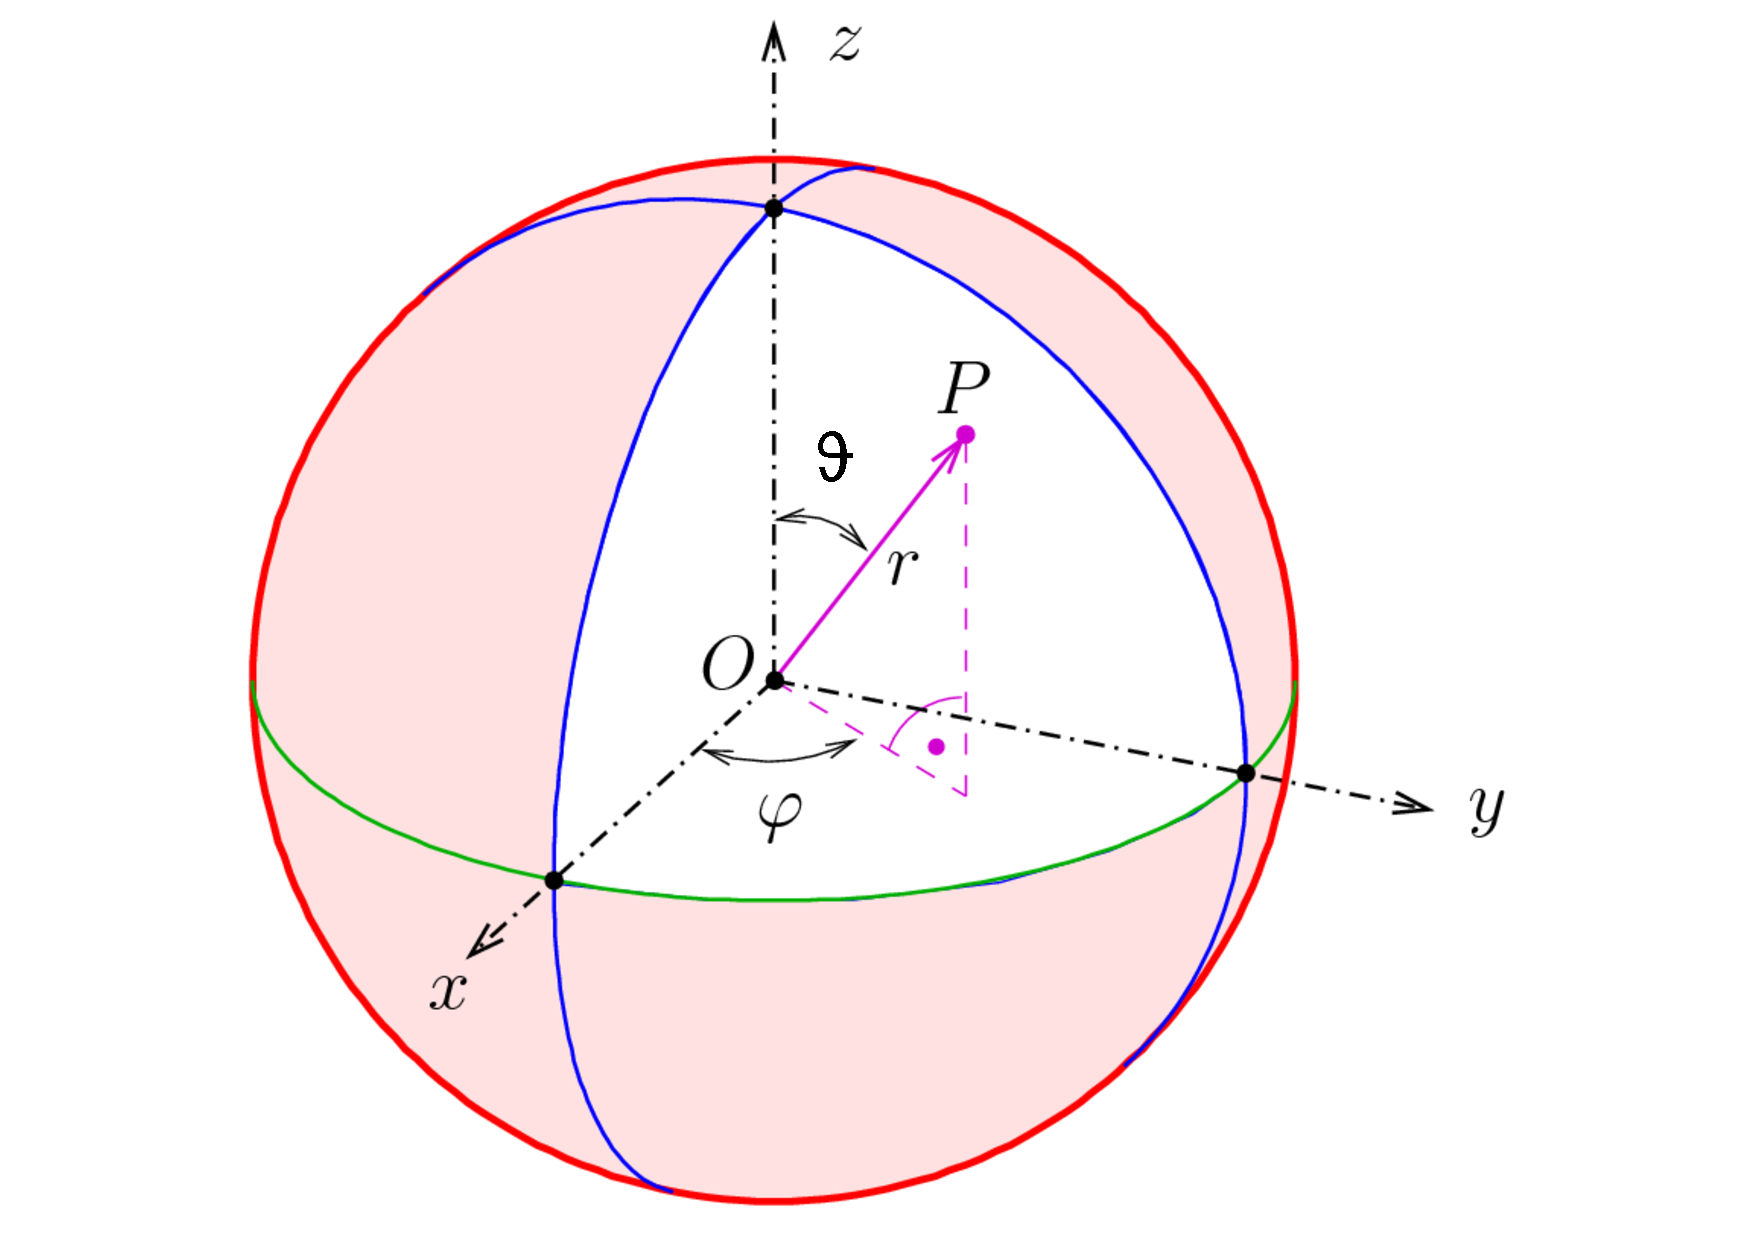
\includegraphics[width=0.7\textwidth]{kugel/Kugelkoord.pdf}
\caption{Koordinaten der Kugel
\label{skript:Koordinaten der Kugel}}
\end{figure}

In der Abbildung \ref{skript:Koordinaten der Kugel} 
ist zu sehen, wie eine Position auf der Kugeloberfl"ache in
Kugel-Koordinaten definiert ist. 
Da wir uns diesem Kapitel  aber nur auf der Oberfl"ache der 
Einheitskugel bewegen wird der Radius r konstant auf 1 gesetzt. 
Durch Variation des Winkels $\vartheta$ ver"andern wir die geographische
Breite und mit dem Winkel $\varphi$ variieren wir die geographische 
L"ange. 
Dadurch l"asst sich jede Position auf der Kugeloberfl"ache definieren. 
Zum Umrechnen ins kartesische Koordinatensystem verwenden wir die 
Formeln:
\[
\left.\begin{aligned}
x& = r \cdot \sin\vartheta \cdot \cos\varphi\\
y& = r \cdot \sin\vartheta \cdot \sin\varphi\\
z& = r \cdot \cos\vartheta\\      
\end{aligned}
\right\}
\qquad (r = 1 \wedge 0 \leq \vartheta \leq \pi \wedge {-\pi} \leq \varphi \leq \pi)
\]

\subsection{Rechteckfunktionen}
\begin{figure}%Funktion auf Rechteckoberfläche 
\centering
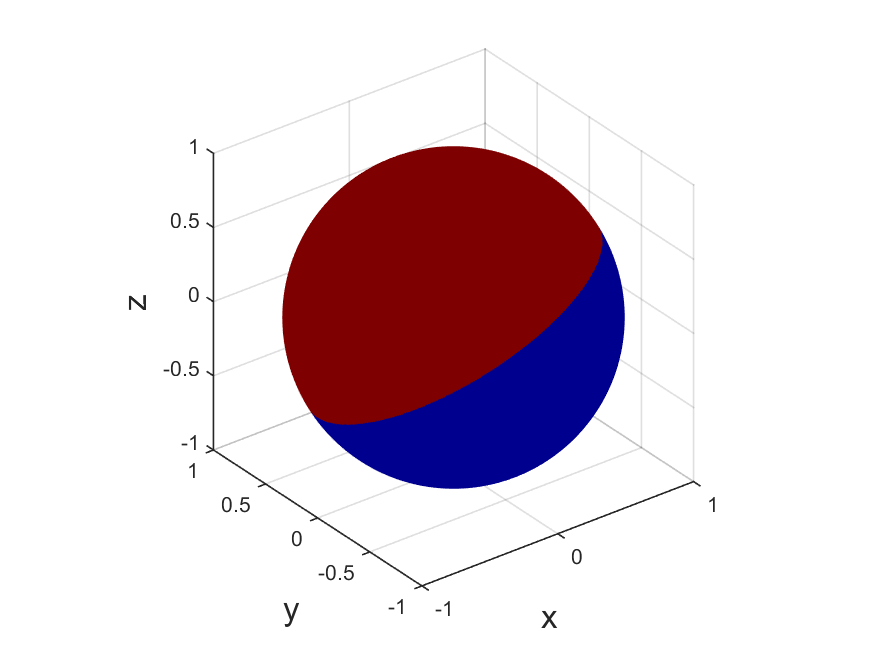
\includegraphics[width=0.5\textwidth]{kugel/Funktion.pdf}
\caption{Funktion auf Kugeloberfl"ache
\label{skript:Funktion auf Kugeloberfl"ache}}
\end{figure}
Die $2\pi$-periodische Rechteckfunktion in unseren Beispielen wird 
mit den Funktionswerten 0 und 1 definiert. 
Die Funktion auf der Kugeloberfl"ache wird analog 
mit denselben Funktionswerten definiert. 
Dabei wird einem kreisf"ormigen Abschnitt auf der Kugeloberfl"ache 
der Wert 1 zugewiesen und der Rest der Kugeloberfl"ache besitzt den 
Funktionswert 0. 

Eine $2\pi$-periodische Rechteckfunktion ist folgendermassen definiert:
\begin{equation}
f(x) =
\begin{cases}
1 & \text{f"ur } u+2\pi k \leq x \leq v + 2\pi k\\
0 & \text{f"ur } 2\pi k \leq x \leq u + 2\pi k \wedge v + 2\pi k \leq x \leq 2\pi (k+1) \\
\end{cases}
\label{skript:Rechteckfunktion Formel}
\end{equation}
$$
k \in \mathbb Z \wedge 0 \leq u \leq 2\pi \wedge u \leq v \leq 2\pi
$$


Das Analogon auf der Kugeloberfl"ache bauen wir wie folgt auf:
\begin{enumerate}
\item Wir definieren einen Vektors $\vec{c}$ mit den Kugel-Koordinaten
$\vartheta_c$ und $\varphi_c$.
Dieser Vektor hat den Startpunkt im Zentrum der Kugel und den Endpunkt 
auf der Kugeloberfl"ache:

\begin{equation}
\vec{c} = 
\begin{pmatrix}
{\sin\vartheta_c \cdot \cos\varphi_c}\\
{\sin\vartheta_c \cdot \sin\varphi_c}\\
{\cos\vartheta_c}
\end{pmatrix}
\label{skript:Vektor c Formel}
\end{equation}
$$
\vartheta_x \in \{0, \pi\} \wedge \varphi_y \in \{-\pi, \pi\}
$$

\item Des Weiteren definieren wir eine Vektorschar $\vec{r}$.
Die zugeh"origen Vektoren $\overrightarrow{r_{xy}}$ haben, wie der 
Vektor $\vec{c}$, die Startpunkte im Zentrum der Kugel und die 
Endpunkte auf der Kugeloberfl"ache. 
Jedoch werden im Gegensatz zu Vektor $\vec{c}$, die Vektoren  
$\overrightarrow{r_{xy}}$ der Vektorschar $r$ mit den Kugelkoordinaten
$\vartheta_x$ und $\varphi_y$ definiert.
\[
\overrightarrow{r_{xy}} = 
\begin{pmatrix}
{\sin\vartheta_x \cdot \cos\varphi_y}\\
{\sin\vartheta_x \cdot \sin\varphi_y}\\
{\cos\vartheta_x}
\end{pmatrix}
\]
$$
0 \leq \vartheta_x \leq \wedge -\pi \leq \varphi_y \leq \pi\
$$

\item Als letztes berechnen wir die Skalarprodukte des Vektors $\vec{c}$
und den Vektoren $\overrightarrow{r_{xy}}$.
Dadurch erh"alt man den Kosinus des Zwischenwinkels des Vektors $\vec{c}$
und dem jeweiligen Vektor $\overrightarrow{r_{xy}}$.
Mit dem Parameter $w$ legt man letztendlich fest, wie gross der 
Kreisabschnitt werden soll, welchem der Wert eins zugewiesen wird.
\begin{equation}
f(\vartheta, \varphi) =\begin{cases}
1 & \text{wenn } \vec{c} \bullet \overrightarrow{r_{xy}} \geq w\\
0 & \text{sonst}
\end{cases}
\label{skript:Kugelfunktion Formel}
\end{equation}
\end{enumerate}
\section{Fourier-Theorie}
\rhead{Fourier-Theorie}
In diesem Abschnitt m"ochten wir die Theorie f"ur die Fourier-Theorie
auf der Kugeloberfl"ache vermitteln. 
Zum einfacheren Verst"andnis, wird immer zuerst die Formel der 
klassischen Fourier-Theorie aufgezeigt, bevor wir die Formel der 
Fourier-Theorie auf der Kugeloberfl"ache darstellen.

\subsection{Kugelfl"achenfunktionen}
Kugelfl"achenfunktionen sind die Analoga zu den Sinus- und 
Kosinus-Funktionen bei der klassischen Fourier-Theorie. 
Mittels dieser Kugelfl"achenfunktionen $Y_{lm}$ und $Z_{lm}$ 
bildet man ein orthogonales System von Funktionen. 
Die Kugelfl"achenfunktionen sind wie folgt definiert:
\begin{align*}
Y_{lm}(\vartheta, \varphi)& = P_{lm} \cdot (\cos \varphi) \cdot \cos(m \cdot \varphi)
\\
Z_{lm}(\vartheta, \varphi)& = P_{lm} \cdot (\cos \varphi) \cdot \sin(m \cdot \varphi)
\end{align*}
Wobei es sich bei $P_{lm}$ um das in Kapitel \ref{skript:legendreansatz} 
hergeleitete Legendre-Polynom handelt. 
Mit $l$ wird der Grad des Legendre-Polynoms angegeben und f"ur $m$
gilt die Bedingung $0 \leq m \leq l$.  
In Abbildung \ref{skript:ylm l=5 m=0} bis \ref{skript:zlm l=5 m=5} sieht man die verschiedenen 
Kugelfl"achenfunktionen vom Grad $l = 5$.

\begin{figure}
\begin{minipage}[hbt]{0.4\textwidth}
\centering
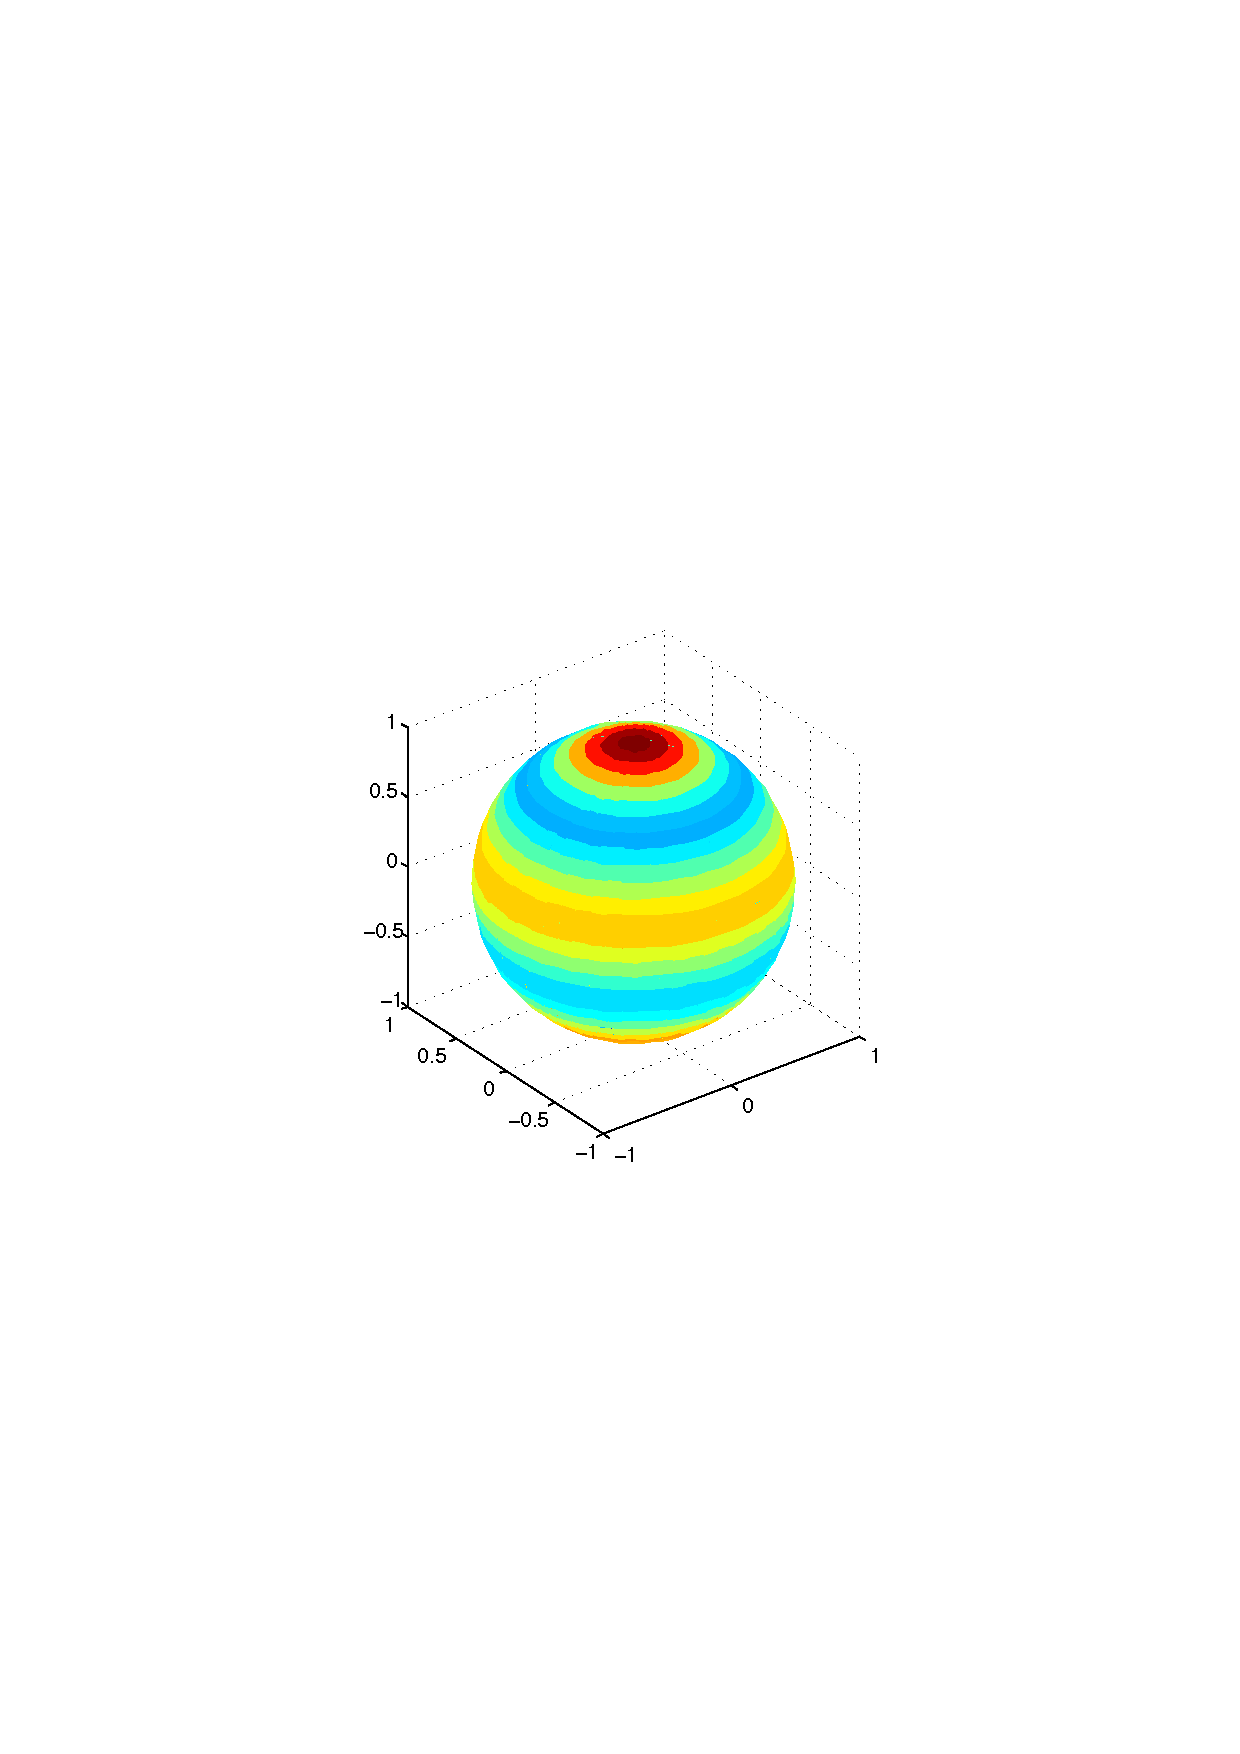
\includegraphics[width=1\textwidth]{kugel/ylm/a_5_0.pdf}
\caption{$Y_{lm}$ mit $l=5$, $m=0$}
\label{skript:ylm l=5 m=0}
\end{minipage}
\hfill
\begin{minipage}[hbt]{0.4\textwidth}
\centering
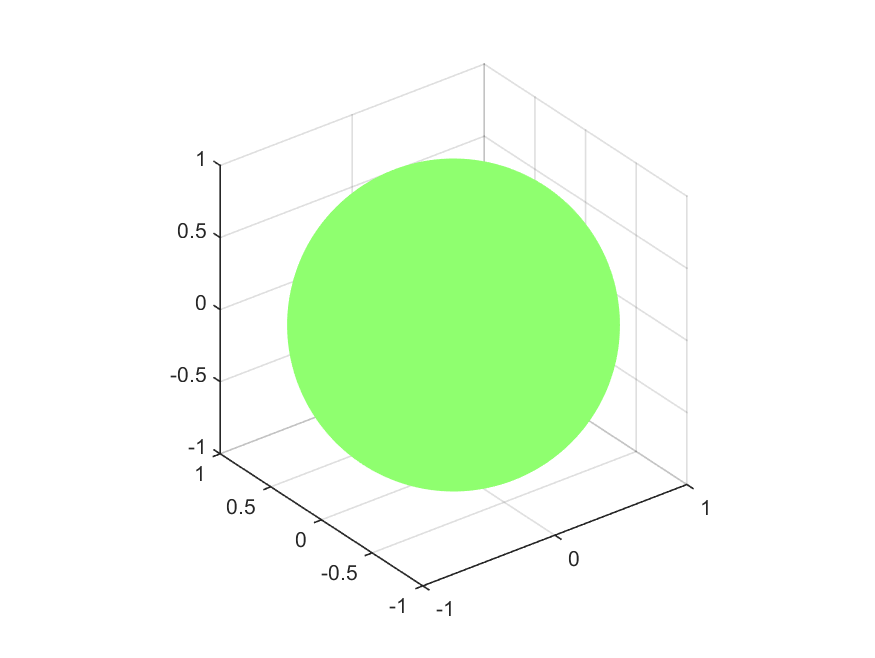
\includegraphics[width=1\textwidth]{kugel/ylm/b_5_0.pdf}
\caption{$Z_{lm}$ mit $l=5$, $m=0$}
\label{skript:zlm l=5 m=0}
\end{minipage}
\begin{minipage}[hbt]{0.4\textwidth}
\centering
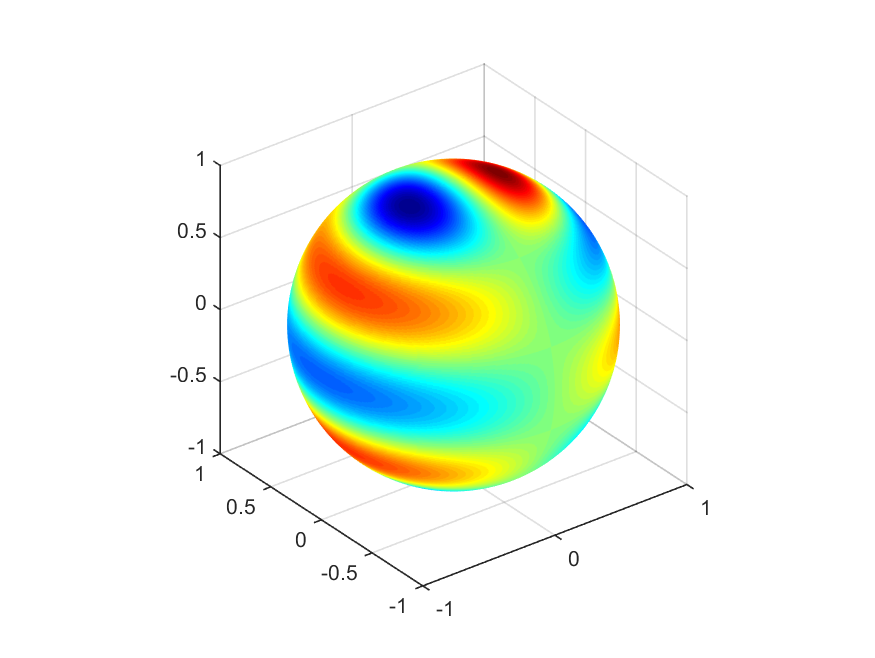
\includegraphics[width=1\textwidth]{kugel/ylm/a_5_1.pdf}
\caption{$Y_{lm}$ mit $l=5$, $m=1$}
\label{skript:ylm l=5 m=1}
\end{minipage}
\hfill
\begin{minipage}[hbt]{0.4\textwidth}
\centering
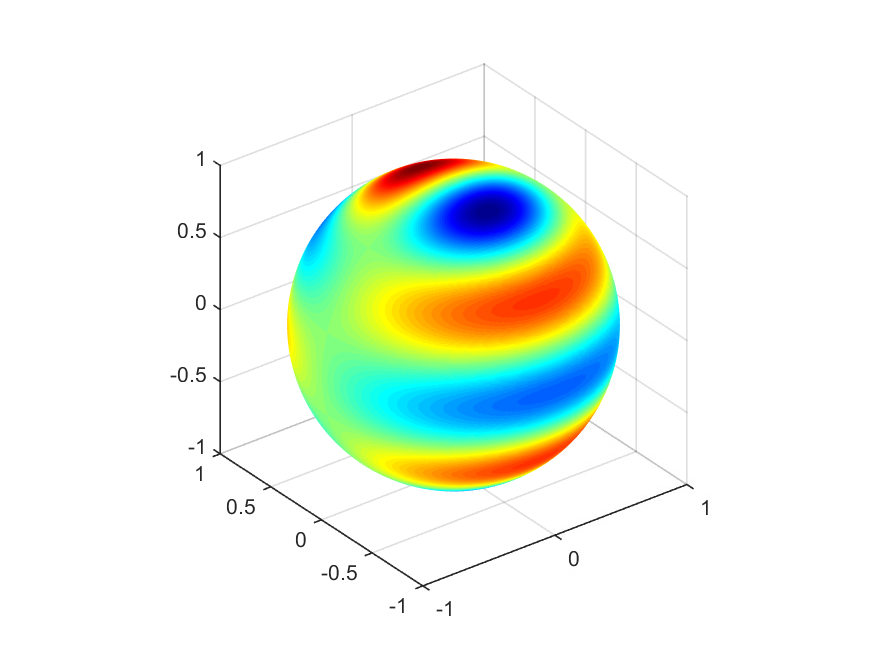
\includegraphics[width=1\textwidth]{kugel/ylm/b_5_1.pdf}
\caption{$Z_{lm}$ mit $l=5$, $m=1$}
\label{skript:zlm l=5 m=1}
\end{minipage}
\begin{minipage}[hbt]{0.4\textwidth}
\centering
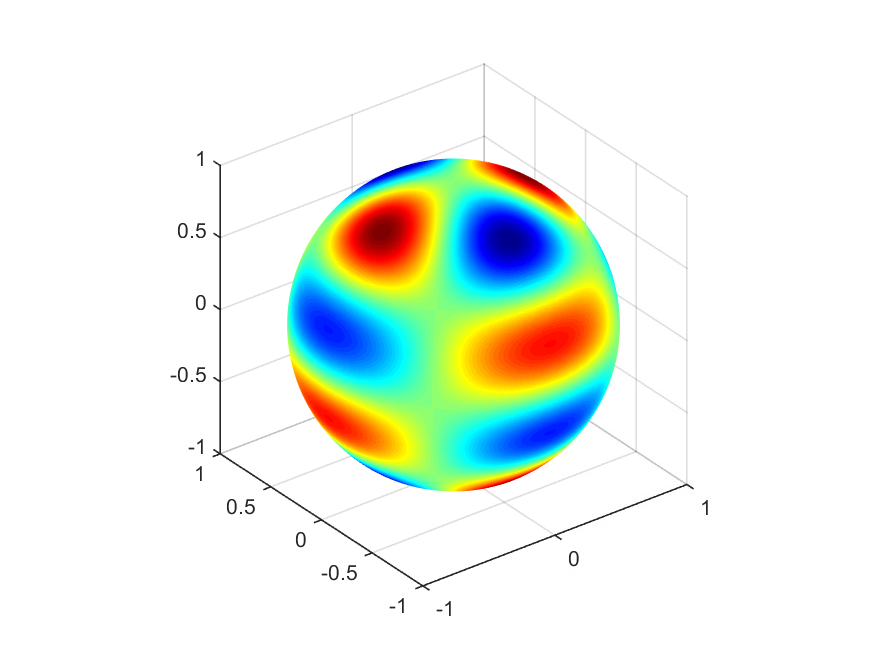
\includegraphics[width=1\textwidth]{kugel/ylm/a_5_2.pdf}
\caption{$Y_{lm}$ mit $l=5$, $m=2$}
\label{skript:ylm l=5 m=2}
\end{minipage}
\hfill
\begin{minipage}[hbt]{0.4\textwidth}
\centering
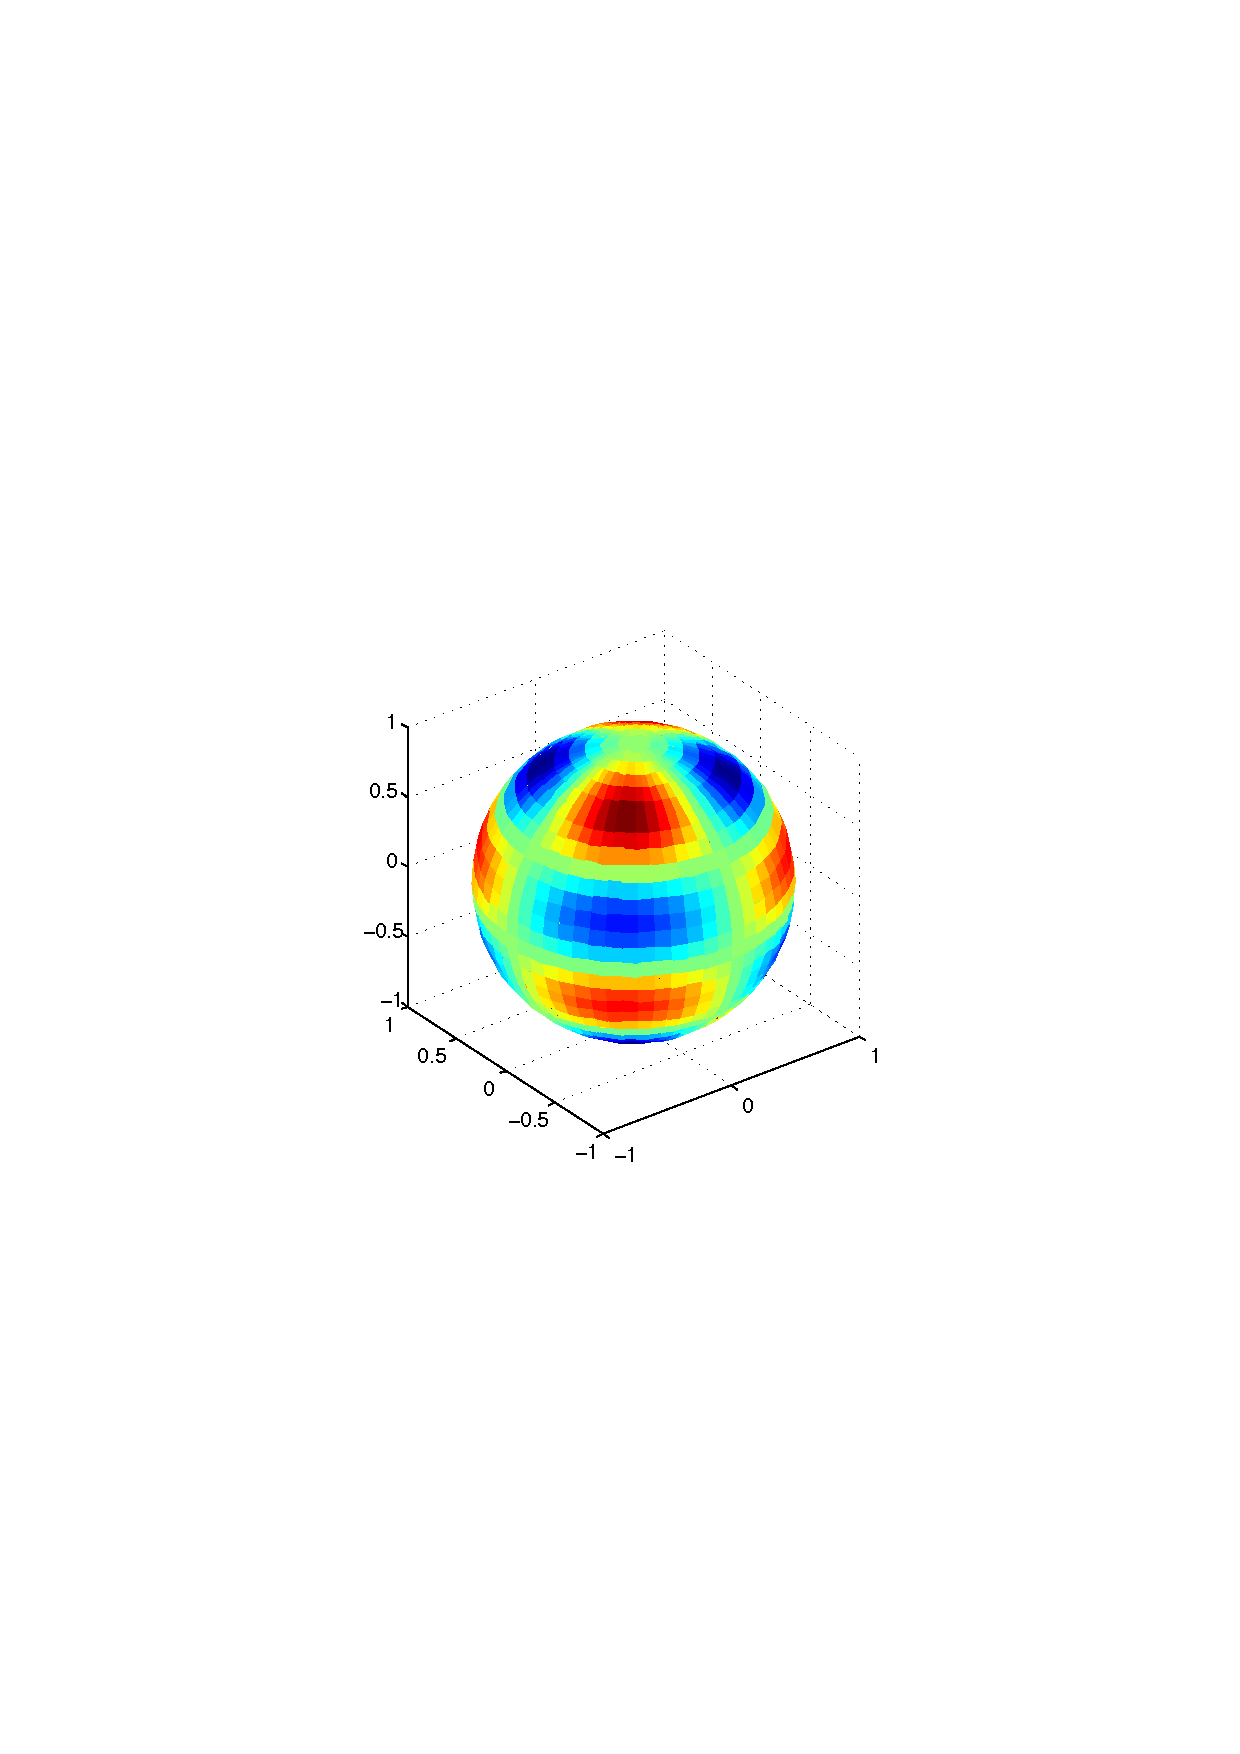
\includegraphics[width=1\textwidth]{kugel/ylm/b_5_2.pdf}
\caption{$Z_{lm}$ mit $l=5$, $m=2$}
\label{skript:zlm l=5 m=2}
\end{minipage}
\end{figure}

\begin{figure}
\begin{minipage}[hbt]{0.4\textwidth}
\centering
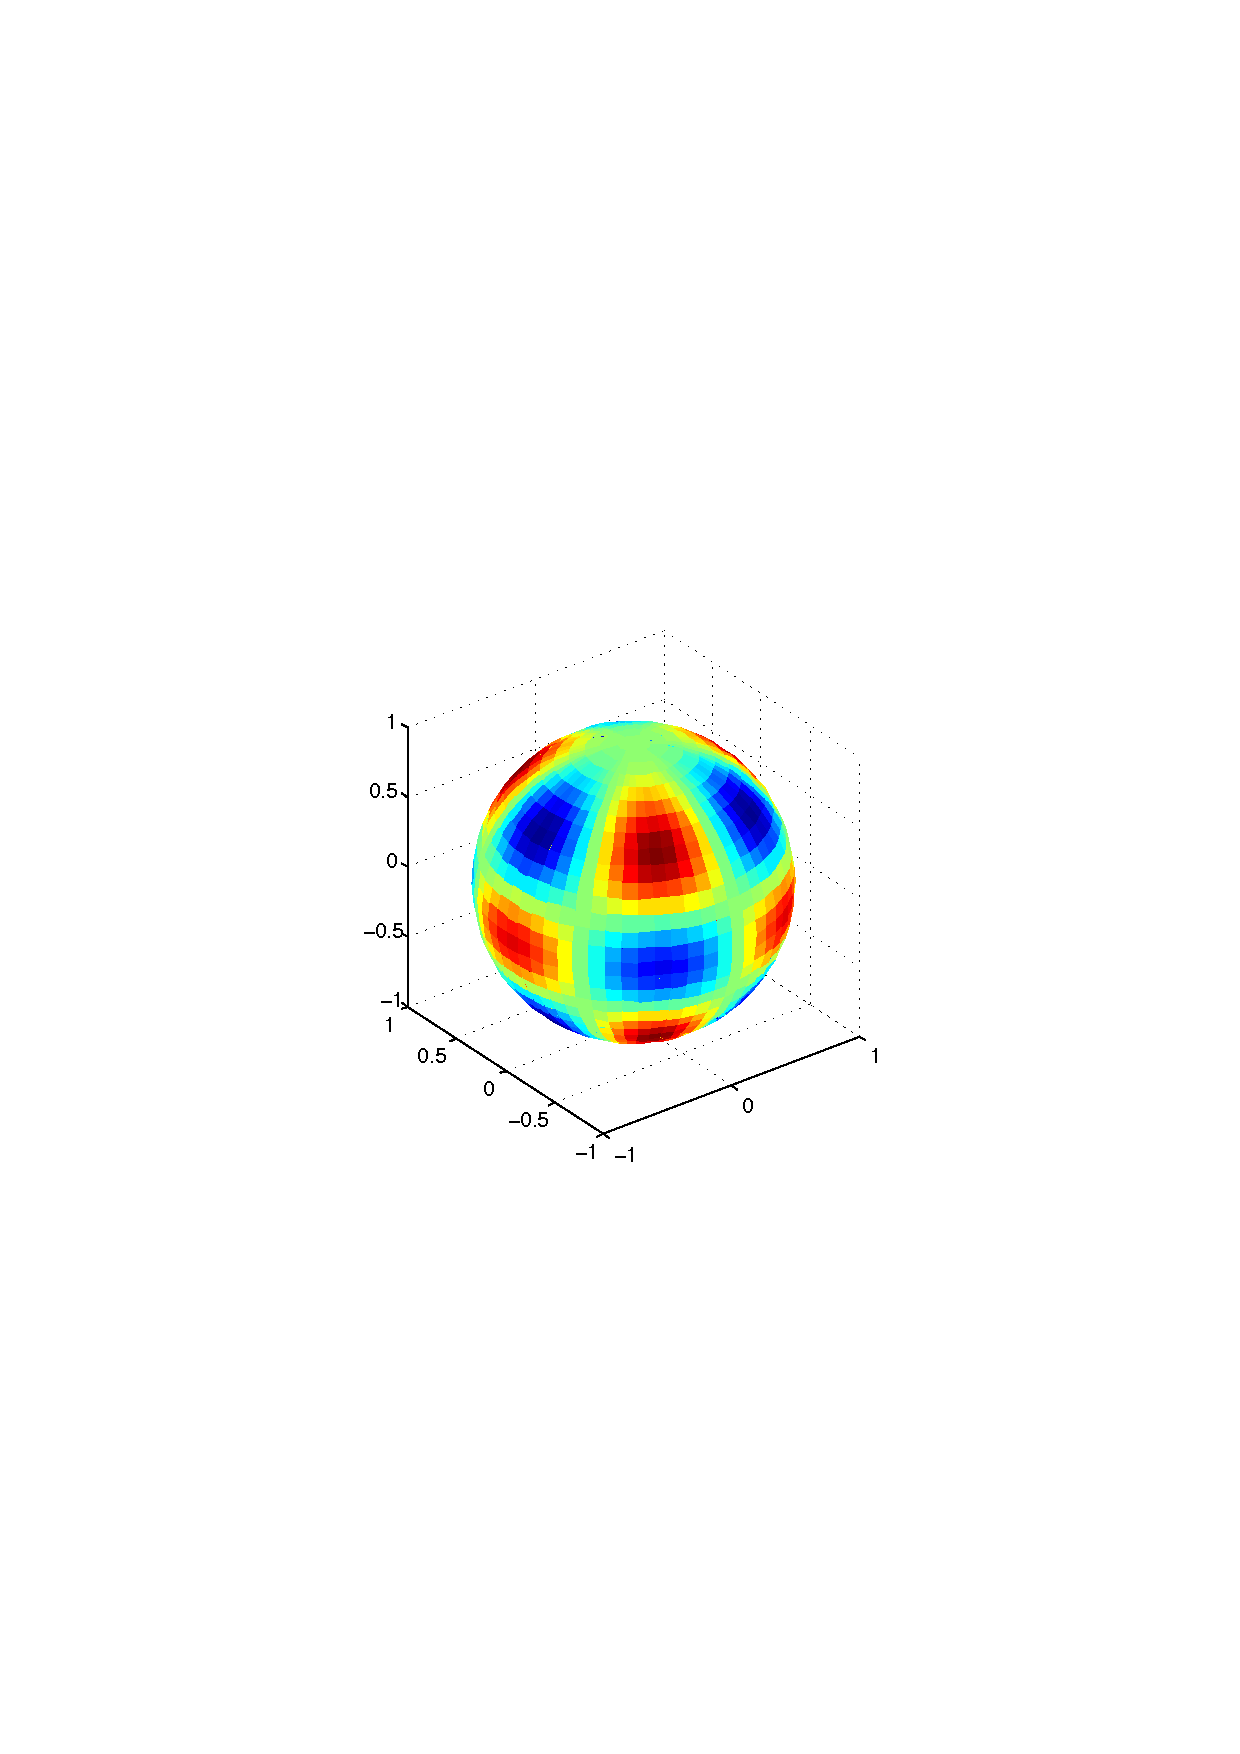
\includegraphics[width=1\textwidth]{kugel/ylm/a_5_3.pdf}
\caption{$Y_{lm}$ mit $l=5$, $m=3$}
\label{skript:ylm l=5 m=3}
\end{minipage}
\hfill
\begin{minipage}[hbt]{0.4\textwidth}
\centering
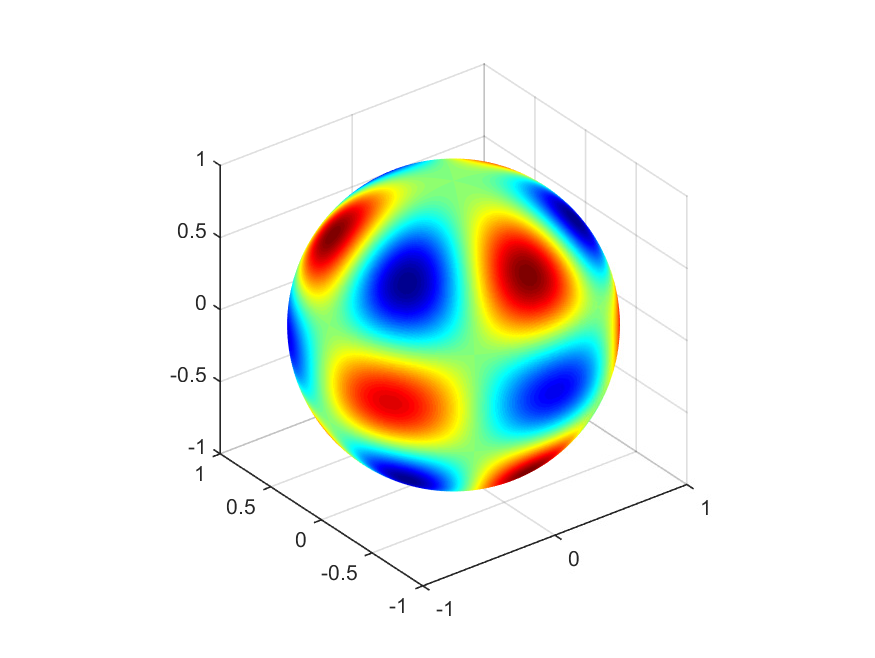
\includegraphics[width=1\textwidth]{kugel/ylm/b_5_3.pdf}
\caption{$Z_{lm}$ mit $l=5$, $m=3$}
\label{skript:zlm l=5 m=3}
\end{minipage}
\begin{minipage}[hbt]{0.4\textwidth}
\centering
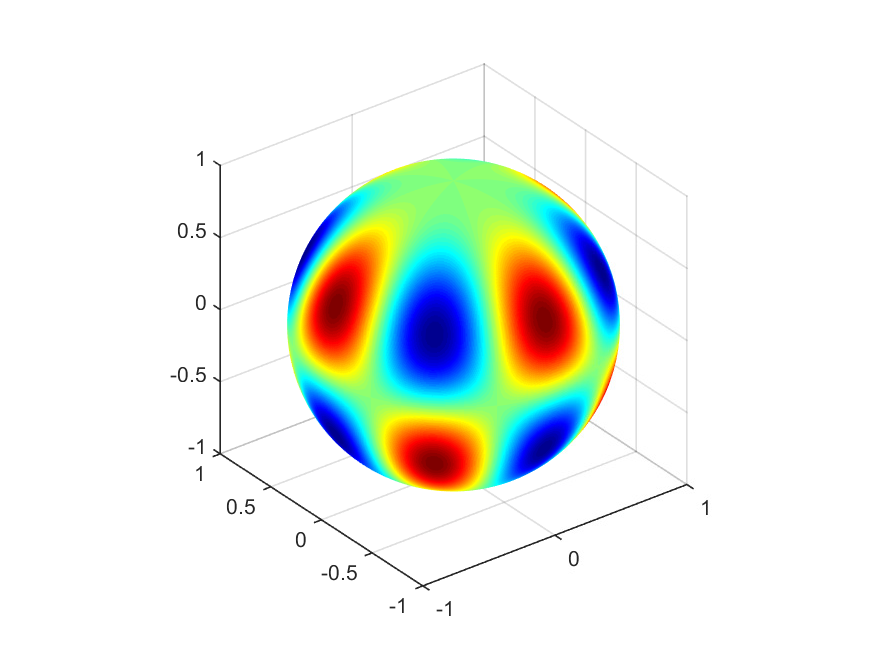
\includegraphics[width=1\textwidth]{kugel/ylm/a_5_4.pdf}
\caption{$Y_{lm}$ mit $l=5$, $m=4$}
\label{skript:ylm l=5 m=4}
\end{minipage}
\hfill
\begin{minipage}[hbt]{0.4\textwidth}
\centering
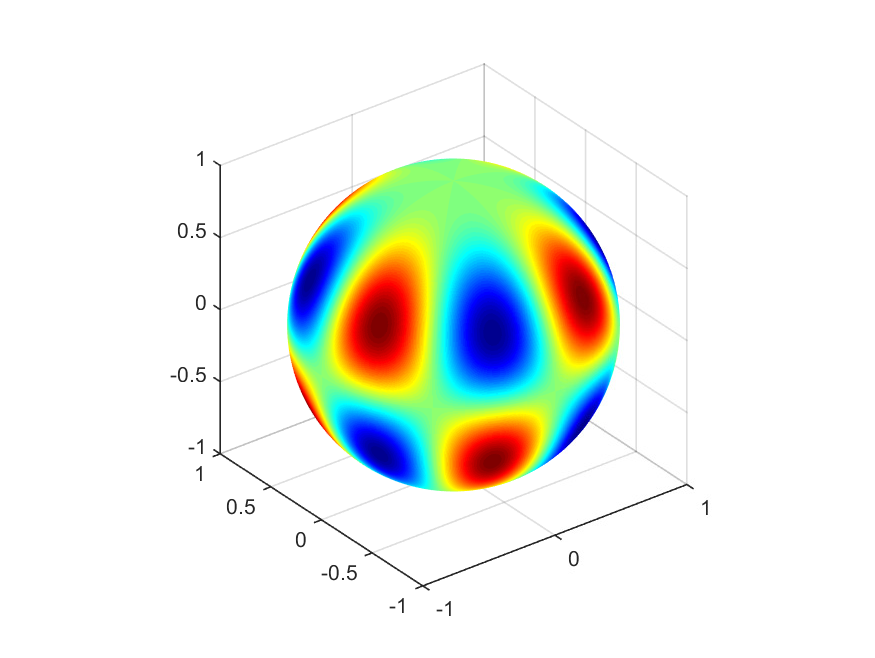
\includegraphics[width=1\textwidth]{kugel/ylm/b_5_4.pdf}
\caption{$Z_{lm}$ mit $l=5$, $m=4$}
\label{skript:zlm l=5 m=4}
\end{minipage}
\begin{minipage}[hbt]{0.4\textwidth}
\centering
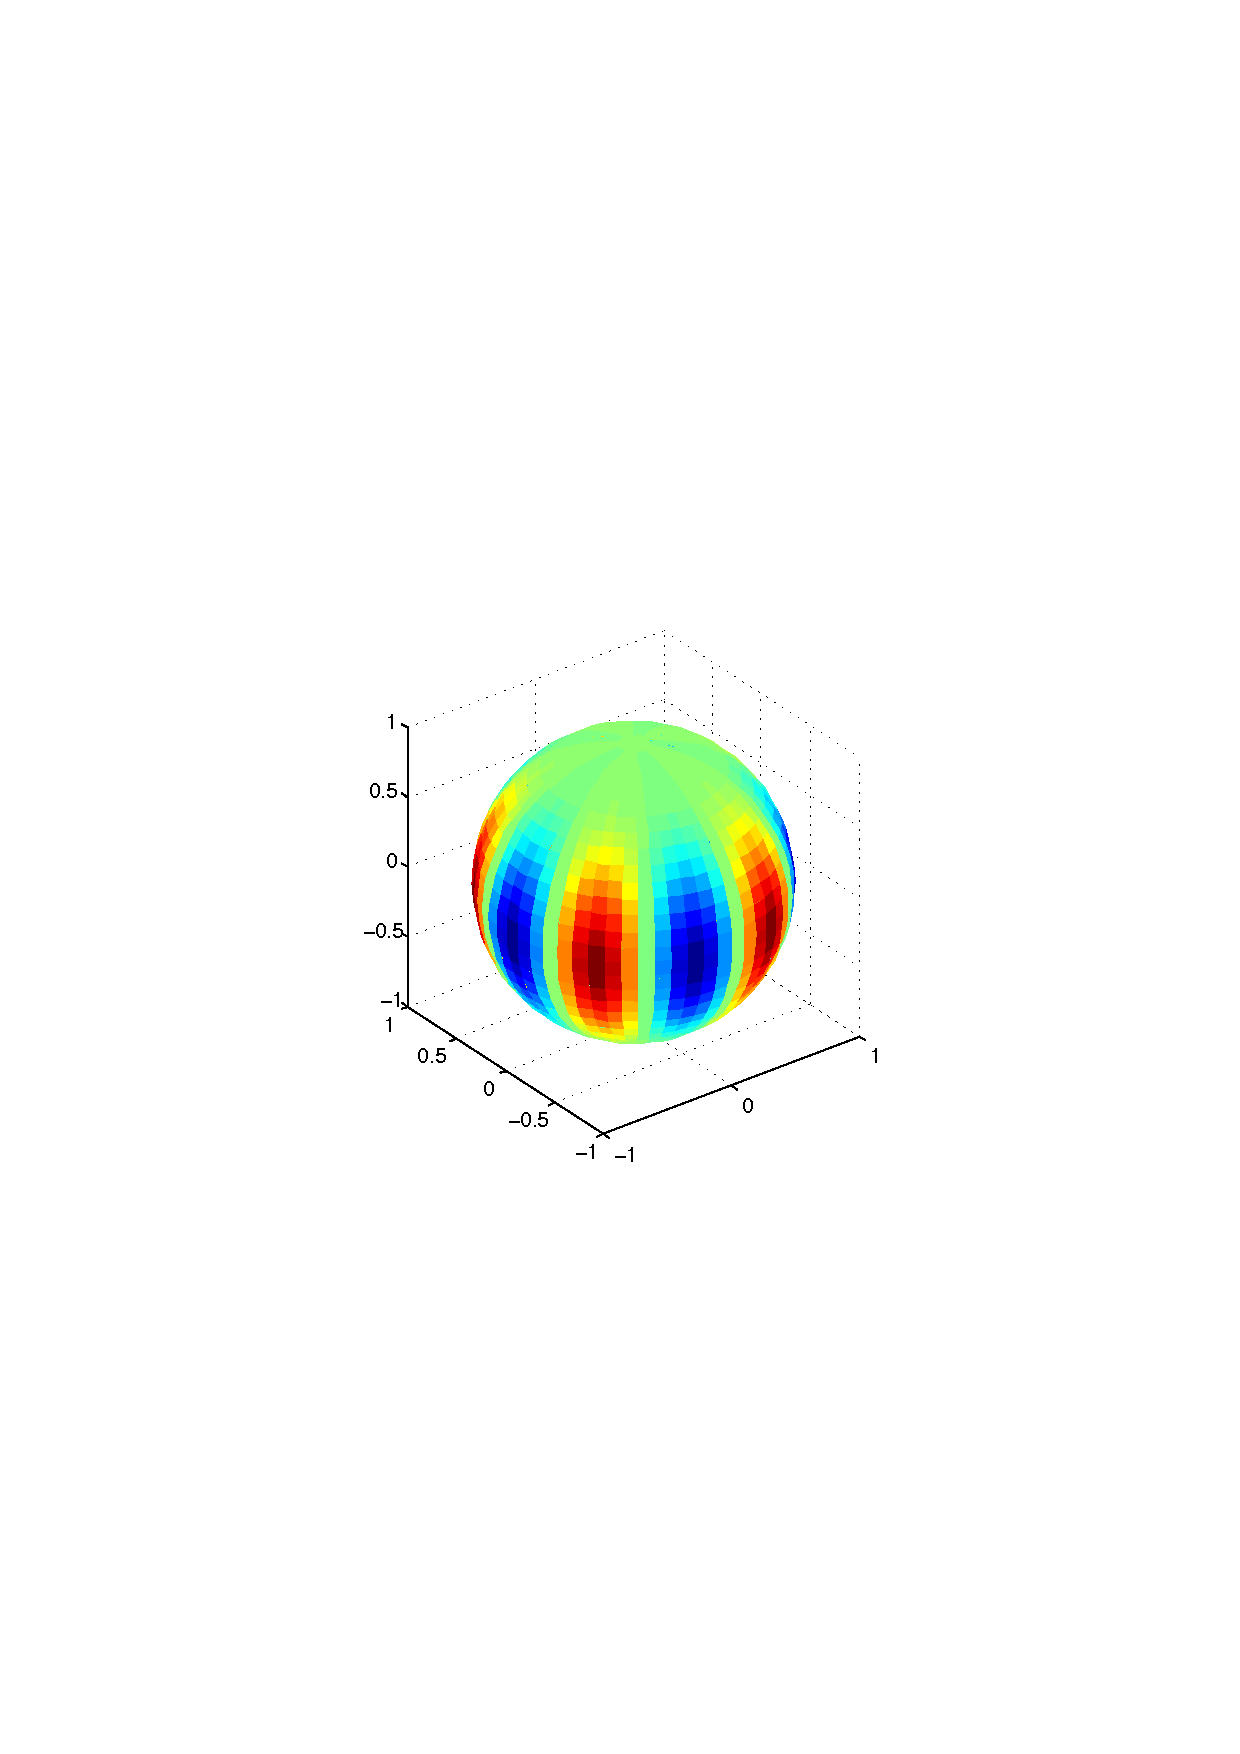
\includegraphics[width=1\textwidth]{kugel/ylm/a_5_5.pdf}
\caption{$Y_{lm}$ mit $l=5$, $m=5$}
\label{skript:ylm l=5 m=5}
\end{minipage}
\hfill
\begin{minipage}[hbt]{0.4\textwidth}
\centering
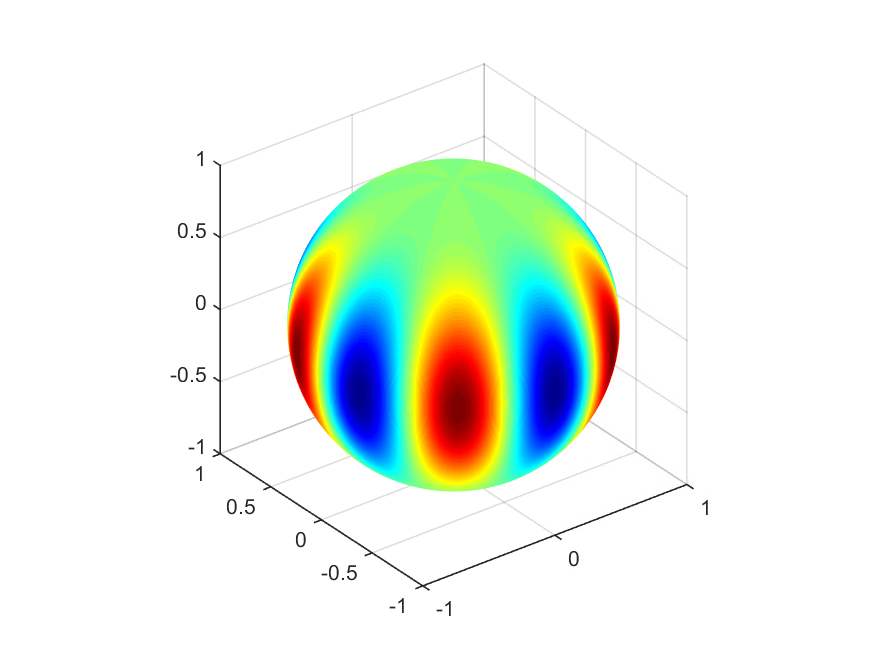
\includegraphics[width=1\textwidth]{kugel/ylm/b_5_5.pdf}
\caption{$Z_{lm}$ mit $l=5$, $m=5$}
\label{skript:zlm l=5 m=5}
\end{minipage}
\end{figure}

\subsection{Fourier-Koeffizienten}
Die Berechnung der Fourier-Koeffizienten in der klassischen 
Fourier-Theorie erfolgt folgendermassen:
\begin{align*}
k&= 0: & a_{0} &= \frac{1}{2\pi} \int_{-\pi}^\pi f(x) \cdot dx
\\
&  & b_{0} &= 0
\\
k& > 0: & a_{k} &= \frac{1}{\pi} \int_{-\pi}^\pi f(x) \cdot \cos kx \cdot dx
\\
& & b_{k} &= \frac{1}{\pi} \int_{-\pi}^\pi f(x) \cdot \sin kx \cdot dx
\end{align*}
F"ur die Berechnung der Fourier-Koeffizienten auf der Kugeloberfl"ache 
verwendet man folgende Formeln:
\begin{align*}
l&=0: & a_{00} &= \frac{1}{4\pi} \int_{-\pi}^\pi \int_{0}^\pi f(\vartheta,\varphi) \cdot \sin\vartheta \cdot d\vartheta \cdot d\varphi
\\
&  & b_{00} &= 0
\\
l&\ne 0: & a_{lm} &= \frac{1}{4\pi} \int_{-\pi}^\pi \int_{0}^\pi f(\vartheta,\varphi) \cdot Y_{lm} (\vartheta, \varphi) \cdot \sin\vartheta \cdot d\vartheta \cdot d\varphi
\\
&  & b_{lm} &= \frac{1}{4\pi} \int_{-\pi}^\pi \int_{0}^\pi f(\vartheta,\varphi) \cdot Z_{lm} (\vartheta, \varphi) \cdot \sin\vartheta \cdot d\vartheta \cdot d\varphi
\end{align*}

\subsection{Berechnung der Funktion aus den Fourier-Koeffizienten}
Um eine Funktion wieder zu rekonstruieren, muss man die einzelnen 
Wellenfunktionen, gewichten mit den entsprechenden Fourier-Koeffizienten 
wieder aufsummieren.

In der klassischen Fourier-Theorie wird folgendermassen vorgegangen:
\begin{equation}
\begin{aligned}
f(x)&=a_0 + \sum_{n=0}^\infty (a_k \cdot \cos kx + b_k \sin kx)
\end{aligned}
\end{equation}
Will man eine Funktion auf der Kugeloberfl"ache wieder rekonstruieren, 
muss man folgende Formel verwenden:
\begin{equation}
\begin{aligned}
f(\vartheta, \varphi) &= a_{00} + \sum_{l=1}^\infty \sum_{m=0}^l (a_{lm} \cdot Y_{lm}(\vartheta, \varphi) + b_{lm} \cdot Z_{lm}(\vartheta, \varphi))
\end{aligned}
\end{equation}
\subsection{Kugelspektrum}
Um das komplexe Amplitudenspektrum darstellen zu k"onnen, muss man die
Sinus- und Kosinus-Koeffizienten noch folgendermassen zusammenfassen:
\begin{align*}
c_k= \sqrt{a^2_{k}+b^2_{k}}
\end{align*}
Analog zum komplexen Amplitudenspektrum kann man ein Kugelspektrum 
darstellen. 
Dabei muss man die Summe der Quadrat $a$- und $b$-Koeffizienten mit 
dem gleichen Index $l$ und $m$. Anschliessend muss man all die Summen
mit dem selben Index $l$ aufsummieren und von den der resultierenden 
Summe die Wurzel ziehen. Diese Schritte werden mittels der folgenden 
Formel realisiert. 
\begin{align*}
c_l= \sqrt{\sum_{m=0}^l (a^2_{lm}+b^2_{lm})}
\end{align*}
Da das Komplexe Amplitudenspektrum sowie das Kugelspektrum enthalten 
keine Ortsinformationen. Dies bedeutet, dass unabh"angig  von der
Phasenlage diese Spektren konstant bleiben, weil die Ortsinformationen
im Phasendiagramm enthalten sind.

\subsection{Nummerische Berechnung des Kugelspektrum}
Allf"allige Abweichungen in unseren Darstellungen sind auf die 
numerischen Berechnungen zur"uckzuf"uhren, da wir mit einer 
Riemann-Summe gerechnet haben.
Qualitativ sind jedoch alle Ergebnisse korrekt. 

\section{Spektrum einer Rechteckfunktion}
\rhead{Spektrum einer Rechteckfunktion}
Um aufzuzeigen, dass das komplexe Amplitudenspektrum unabh"angig der 
Phasenlage konstant bleibt, haben wir eine wandernde Rechteckfunktion 
generiert. 
Dazu variierten die Parameter $u$ und $v$ der Formel 
\ref{skript:Rechteckfunktion Formel}
unter der Bedingung: $u$ - $v$ = $\pi$.
Damit stellten wir sicher, dass die Abmessungen unserer 
Rechteckfunktion konstant bleiben und sich nur die Phasenlage "andert.
In Abbildung \ref{skript:Spektrum1} sieht man eine solche 
Rechteckfunktion in vier verschiedenen Phasenlagen mit den zugeh"origen 
komplexen Amplitudenspektren. 
Es muss beachtet werden, dass beim komplexen Amplitudenspektrum der 
Fourier-Koeffizient $c_0$ aus Darstellungsgr"unden Abgeschnitten wurde.

Um die Analogie f"ur eine Funktion auf der Kugeloberfl"ache aufzuzeigen, 
variierten wir den Vektor $\vec{c}$ indem wir die Winkel $\vartheta_0$
und $\varphi_0$ aus der Formel \ref{skript:Vektor c Formel} 
kontinuierlich ver"anderten. 
Mittels dieser "Anderung variierten wir die Phasenlage. 
Um zu garantieren, dass die Abmessung unserer Funktion konstant bleibt, 
stellten wir die Bedingung dass der Parameter $w$ der Formel 
\ref{skript:Kugelfunktion Formel} konstant auf 0 gesetzt ist. 
Dadurch erhielten wir eine Funktion, welche auf der einen 
H"alfte der Kugeloberfl"ache den Funktionswert 1 und auf der 
anderen H"alfte den Funktionswert 0 besitzt. In Abbildung 
\ref{skript:Spektrum2} sieht man,wie schon bei der Rechteckfunktion, 
unsere Kugelfunktion in vier verschiedenen Phasenlagen und die 
zugeh"origen Kugelspektren.

Um dies noch besser zu veranschaulichen, ist dem Buch eine CD 
beigelegt, auf welcher je ein Video eine wandernde 
Rechteckfunktion mit dem komplexen Amplitudenspektrum, sowie eine 
rotierende Funktion auf der Kugeloberfl"ache mit den zugeh"origen 
Kugelspektrum zu sehen sind. Zus"atzlich sieht man in den Videos auch
die sich st"andig "andernden $a$- und $b$-Koeffizienten und bei der 
Rechteckfunktion ist auch noch das Phasendiagramm dargestellt.

\begin{figure}
\centering
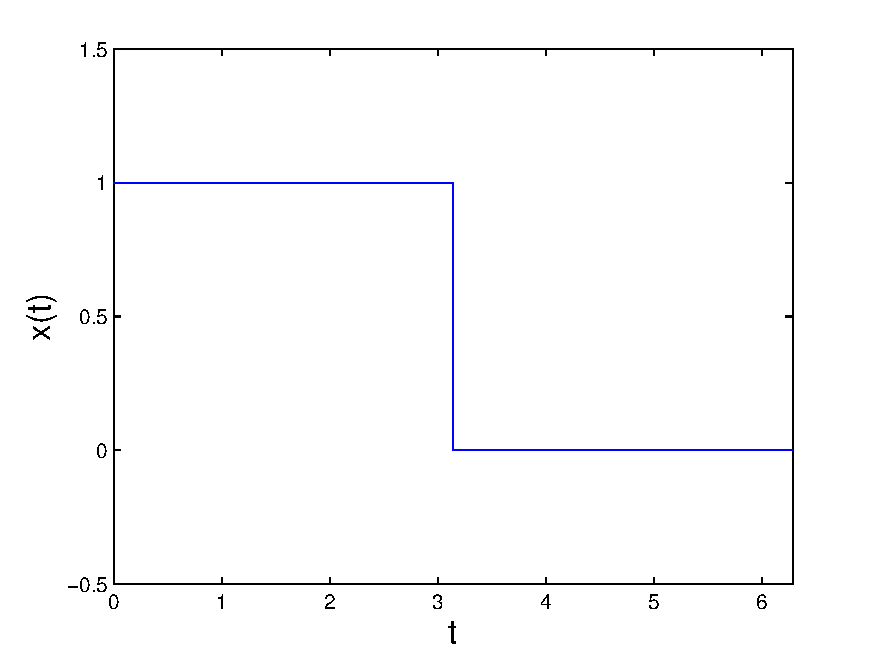
\includegraphics[width=0.45\textwidth]{kugel/kSpektrum/Rechteck1_1.pdf}
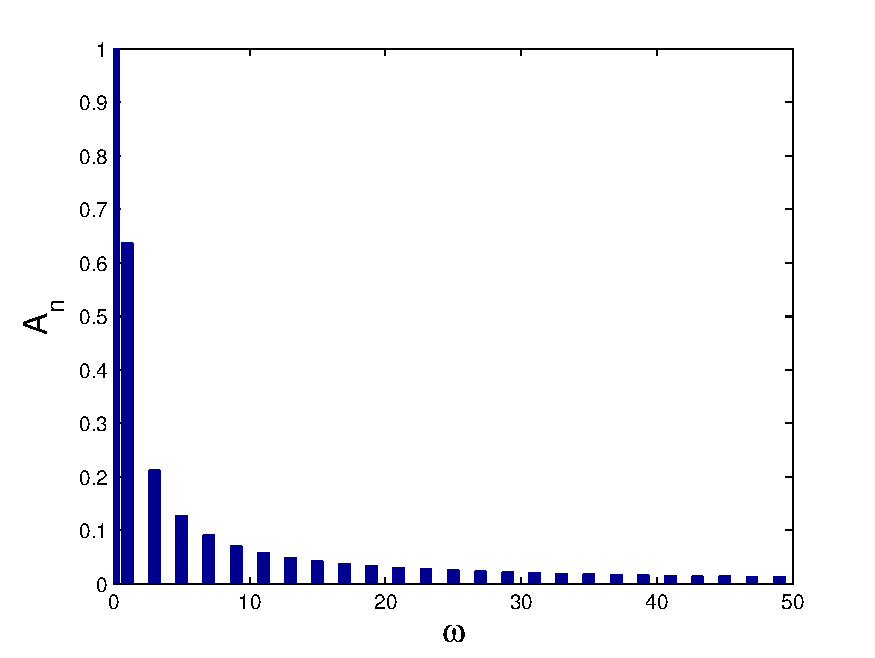
\includegraphics[width=0.45\textwidth]{kugel/kSpektrum/Rechteck1_2.pdf}
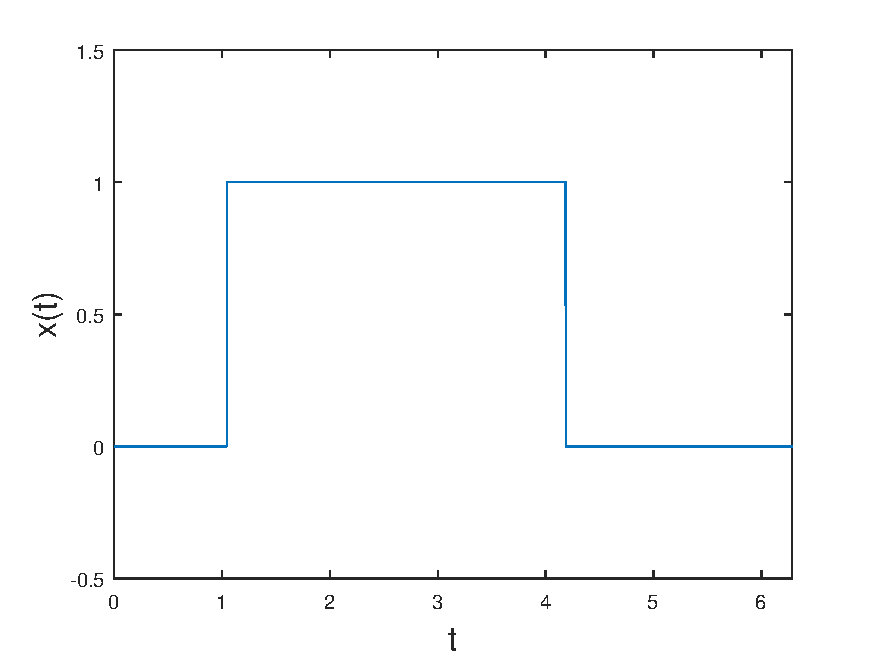
\includegraphics[width=0.45\textwidth]{kugel/kSpektrum/Rechteck2_1.pdf}
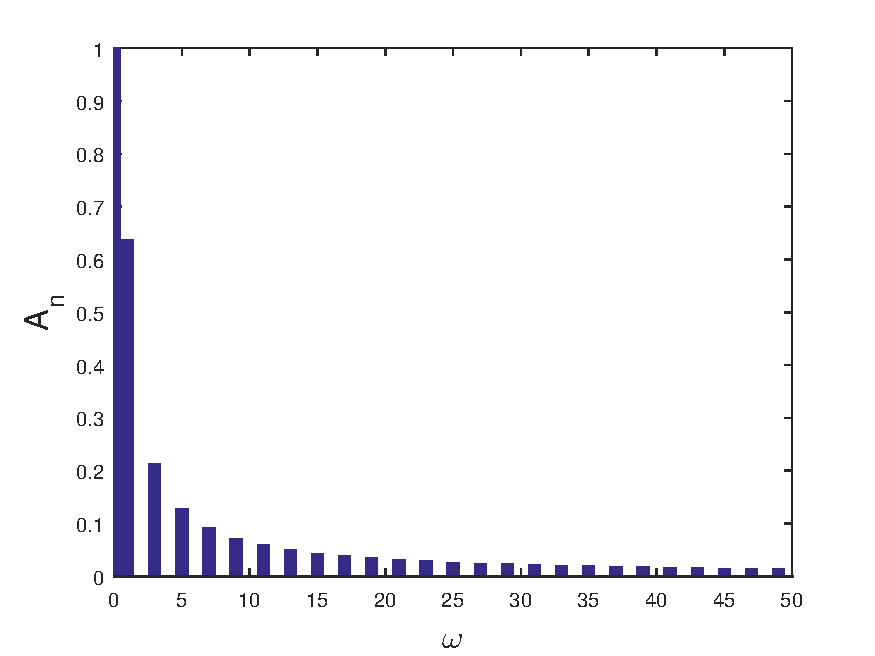
\includegraphics[width=0.45\textwidth]{kugel/kSpektrum/Rechteck2_2.pdf}
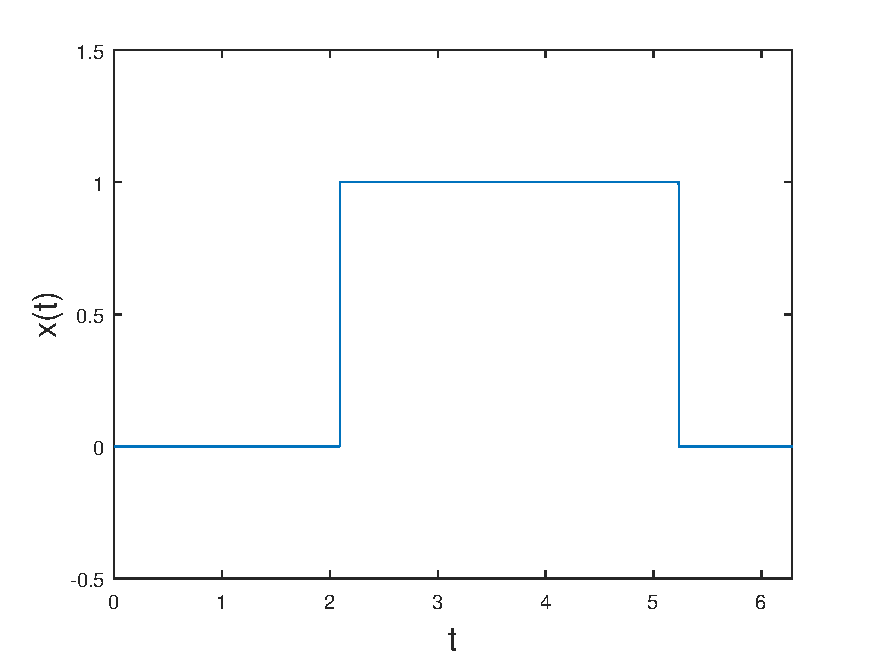
\includegraphics[width=0.45\textwidth]{kugel/kSpektrum/Rechteck3_1.pdf}
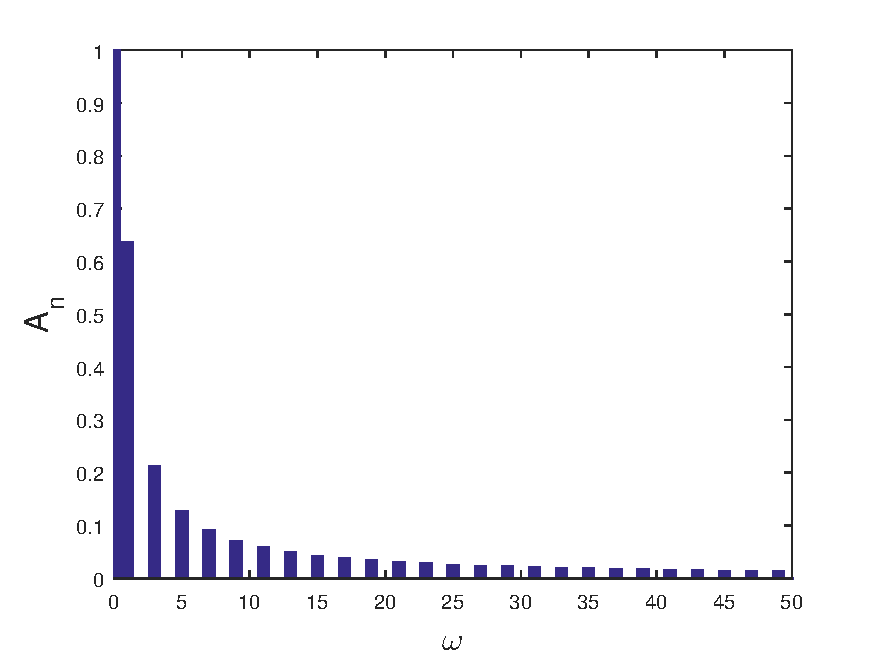
\includegraphics[width=0.45\textwidth]{kugel/kSpektrum/Rechteck3_2.pdf}
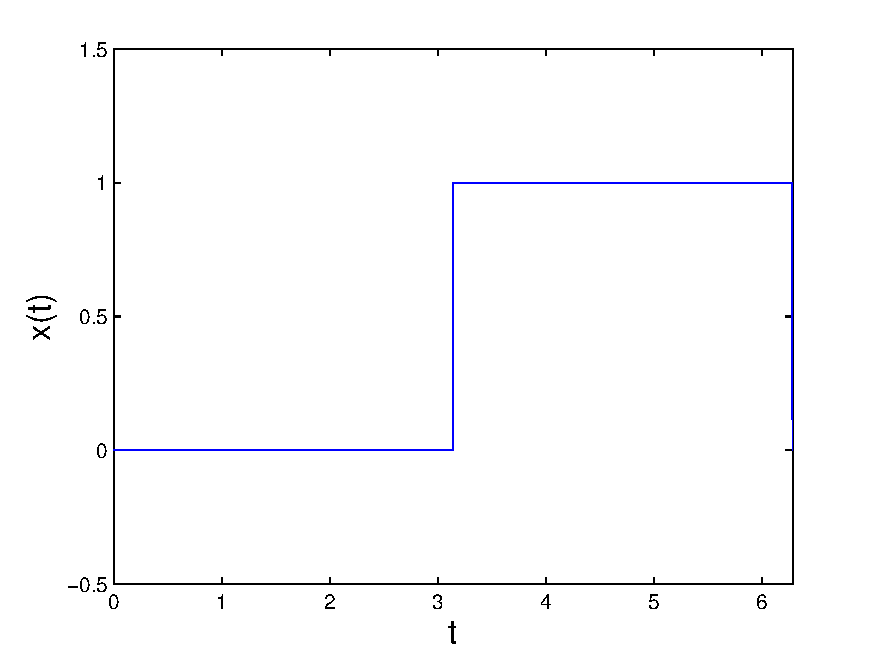
\includegraphics[width=0.45\textwidth]{kugel/kSpektrum/Rechteck4_1.pdf}
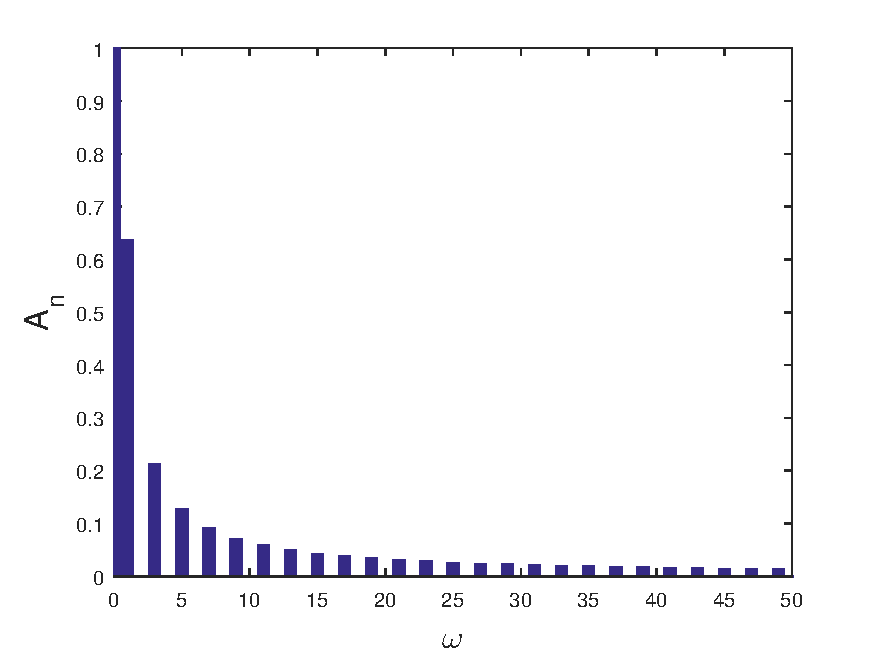
\includegraphics[width=0.45\textwidth]{kugel/kSpektrum/Rechteck4_2.pdf}
\caption{Wandernde Rechteckfunktion
\label{skript:Spektrum1}}
\end{figure}
Dasselbe gilt auch f"ur Funktionen auf der Kugeloberfl"ache, wie man
auf den folgenden Bildern sehen kann.
\begin{figure}
\centering
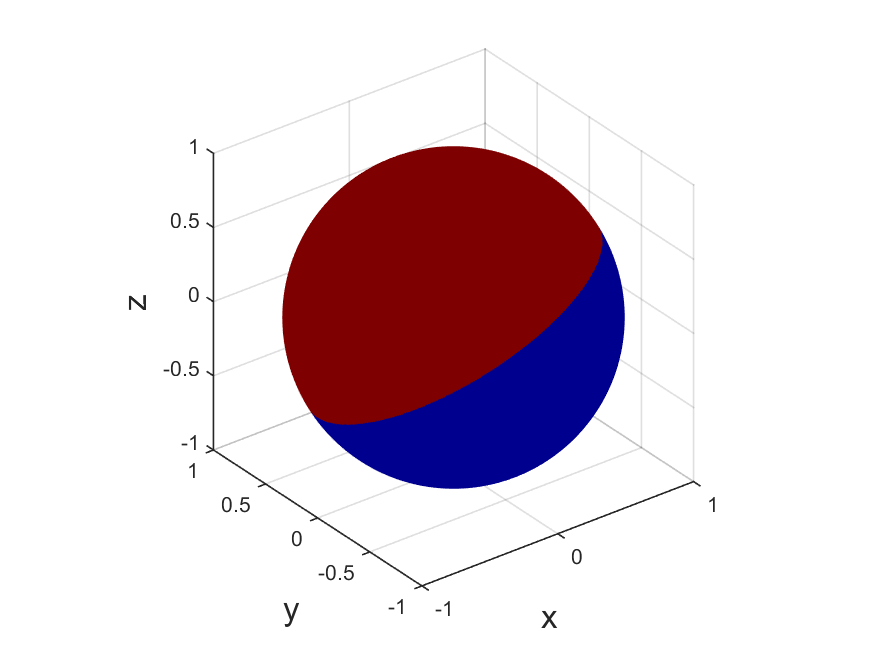
\includegraphics[width=0.45\textwidth]{kugel/kSpektrum/Kugel_1_1.pdf}
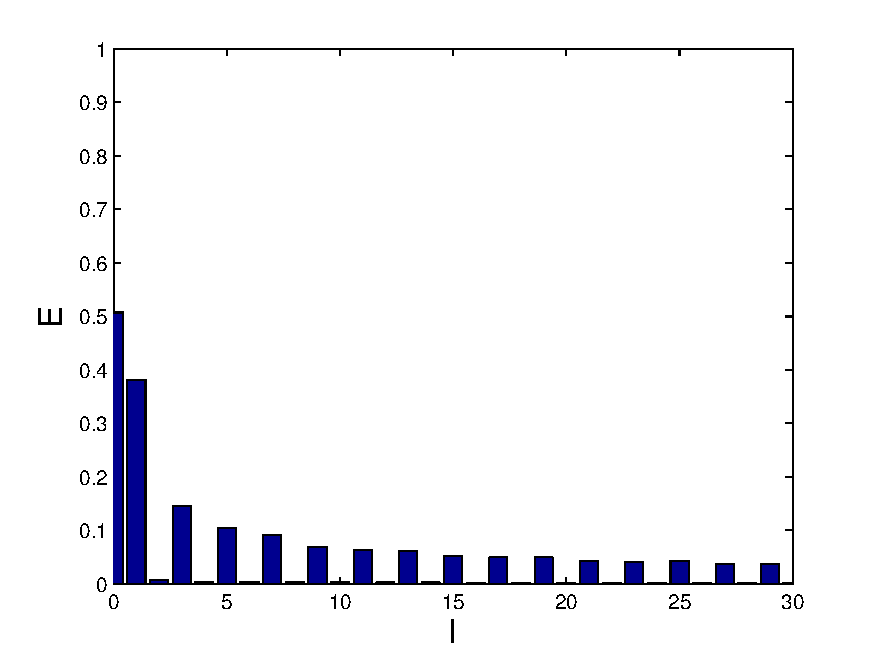
\includegraphics[width=0.45\textwidth]{kugel/kSpektrum/Kugel_1_2.pdf}
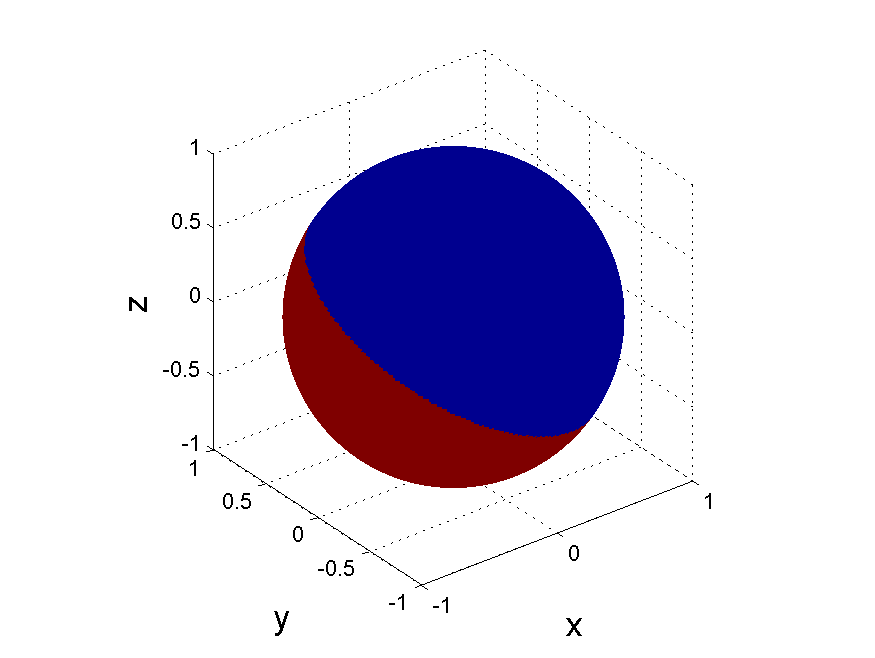
\includegraphics[width=0.45\textwidth]{kugel/kSpektrum/Kugel_2_1.pdf}
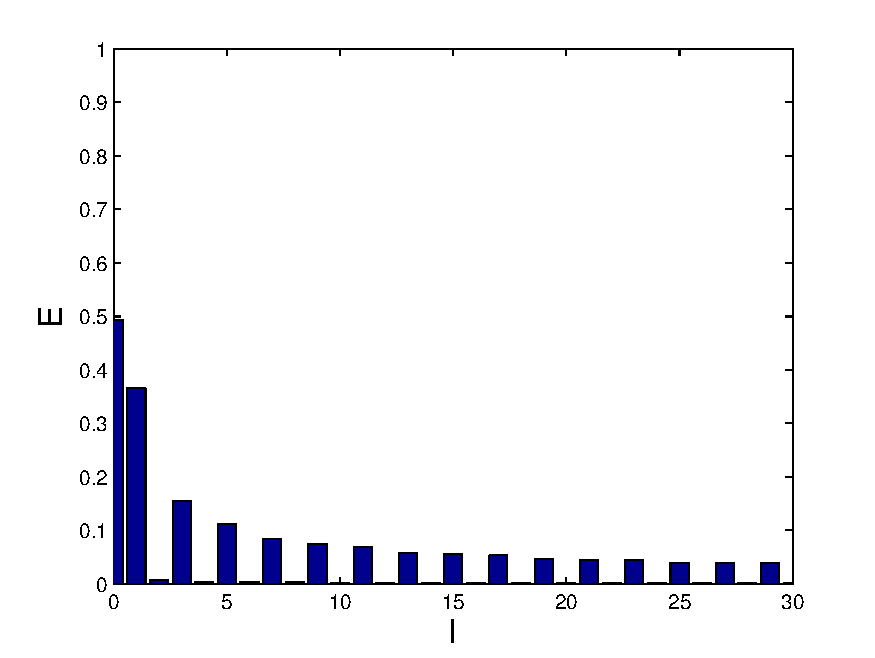
\includegraphics[width=0.45\textwidth]{kugel/kSpektrum/Kugel_2_2.pdf}
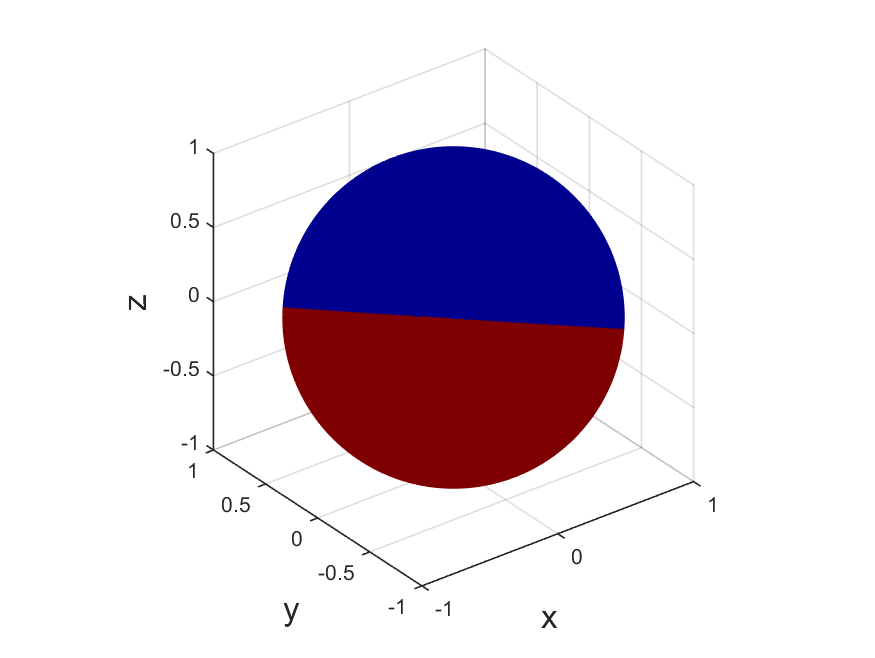
\includegraphics[width=0.45\textwidth]{kugel/kSpektrum/Kugel_3_1.pdf}
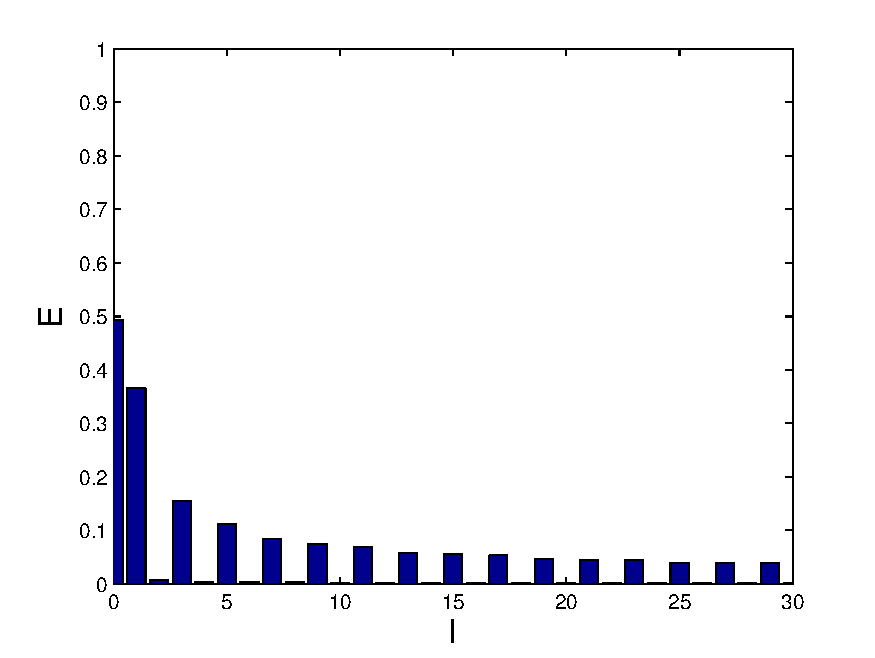
\includegraphics[width=0.45\textwidth]{kugel/kSpektrum/Kugel_3_2.pdf}
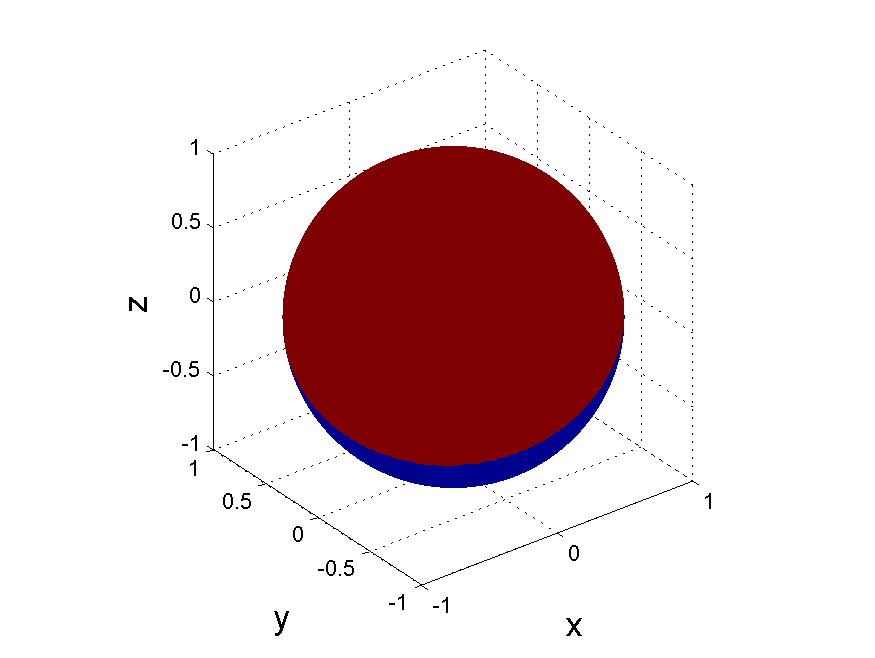
\includegraphics[width=0.45\textwidth]{kugel/kSpektrum/Kugel_4_1.pdf}
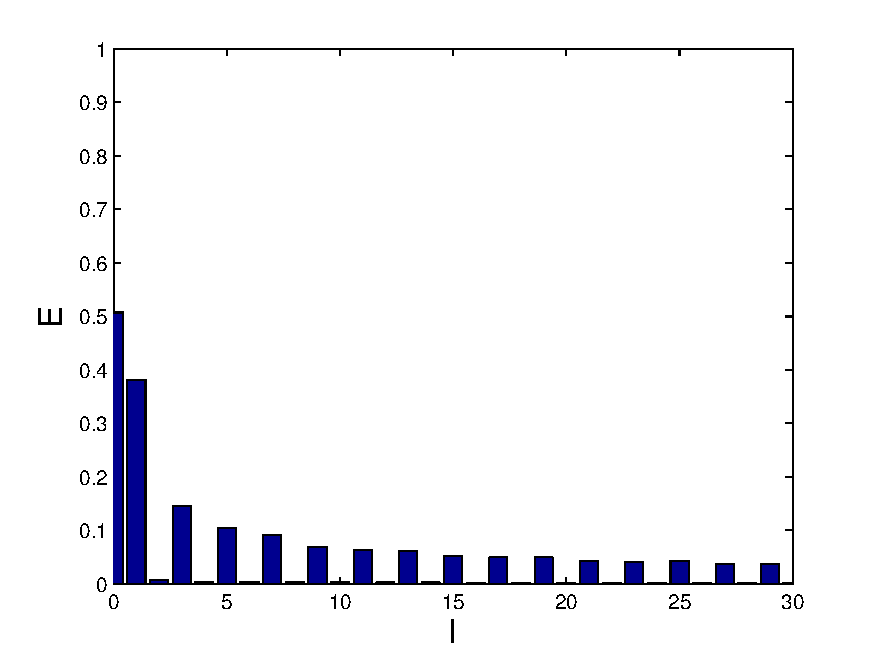
\includegraphics[width=0.45\textwidth]{kugel/kSpektrum/Kugel_4_2.pdf}
\caption{Rotierende Funktion auf der Kugeloberfl"ache
\label{skript:Spektrum2}}
\end{figure}

\section{Dirac Stoss und konstante Funktion}
\rhead{Dirac Stoss und konstante Funktion}

In diesem Abschnitt, m"ochten wir aufzeigen, dass im Falle eines 
unendlich schmalen Rechtecksignals, wie auch einem unendlich kleinen 
Kreisabschnitt auf der Kugeloberfl"ache mit dem Funktionswert 1 beim 
komplexen Amplitudenspektrum und dem Kugelspektrum alle 
Fourier-Koeffizienten gleich stark gewichtet sind. Wenn man hingegen 
ein Rechtecksignal, oder eine Funktion auf der Kugeloberfl"ache, welche 
"uberall den Funktionswert 1 besitzt, analysiert, ist nur noch der 
Fourier-Koeffizient $c_0$ $\neq$ 0.

Um dies für das Rechtecksignal darzustellen, hielten wir den Parameter
$u$ aus der Formel \ref{skript:Rechteckfunktion Formel} konstant auf 0 
und variierten den Parameter $v$ derselben Formel von 0 bis 2$\pi$. 
Dadurch erhielten wir eine immer breiter werdende Rechteckfunktion. 
In Abbildung \ref{skript:Dirac1} sieht man die Rechteckfunktion in 
vier verschiedene Breiten mit den zugeh"origen komplexen 
Amplitudenspektren. 
Wie auch schon bei den komplexen Amplitudenspektren in Abbildung
\ref{skript:Spektrum1} ist der Fourier-Koeffizient $c_0$ aus 
Darstellungsgr"unden abgeschnitten.

Um dies analog auch auf der Kugeloberfl"ache zu illustrieren, hielten 
wir den die Winkel aus der Formel \ref{skript:Vektor c Formel} 
$\vartheta_c$ und $\varphi_c$ konstant und variierten lediglich den 
Parameter $w$ aus der Formel \ref{skript:Kugelfunktion Formel} 
zwischen von 1 bis -1. 
Dadurch wird der Kreisabschnitt welcher den Funktionswert 1 hat immer 
gr"oösser. 
In Abbildung \ref{skript:Dirac2} sieht man die Funktion auf der 
Kugeloberfl"ache mit vier verschieden grossen Kreisabschnitten, welche 
den Funktionswert 1 haben mit den zugeh"origen Kugelspektren.

Um auch dies noch besser zu veranschaulichen, Sind auf der CD zum Buch 
je ein Video mit einer immer Breiter werdenden Rechteckfunktion mit dem 
komplexen Amplitudenspektrum, sowie eine Funktion auf der 
Kugeloberfl"ache mit immer gr"osser werdendem Kreisabschnitt mit 
Funktionswert 1 mit dem zugeh"origen Kugelspektrum zu sehen. 
Wie bei den Videos, welche im letzten Abschnitt erw"ahnt wurden sind 
wieder zus"atzlich die $a$- und $b$-Koeffizienten und bei der 
Rechteckfunktion das Phasendiagramm zu sehen.
\begin{figure}
\centering
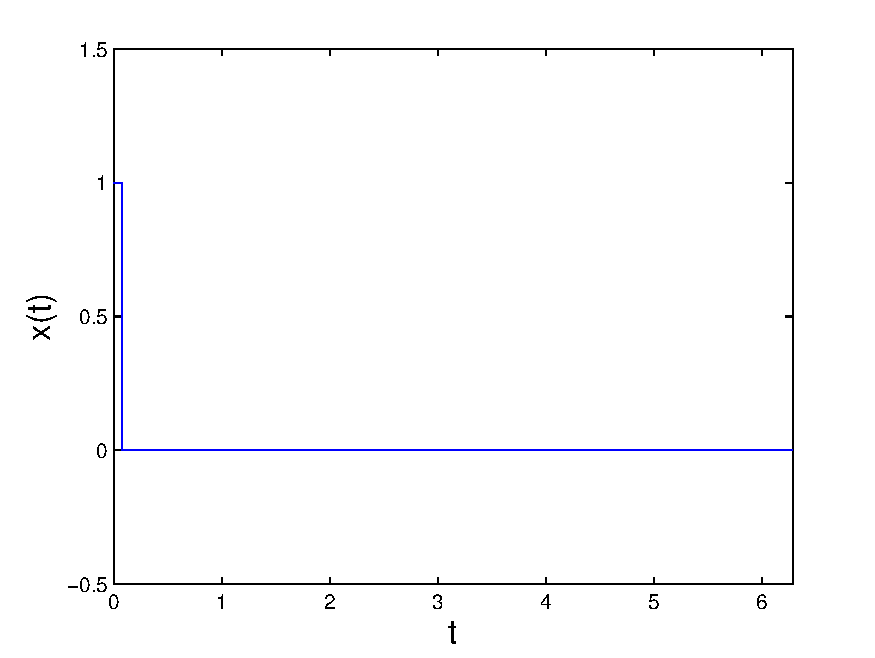
\includegraphics[width=0.45\textwidth]{kugel/Dkonstant/Rechteck1_1.pdf}
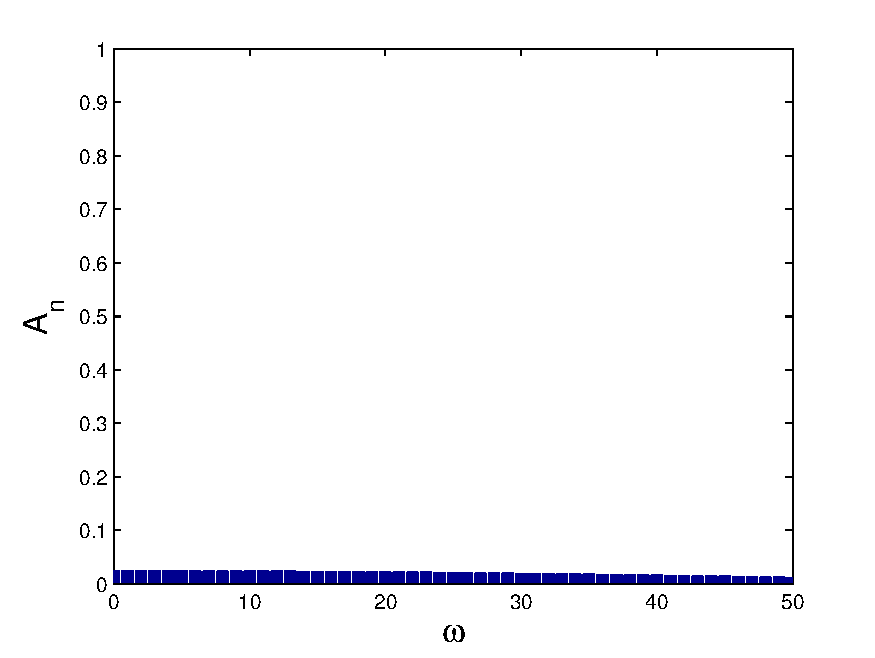
\includegraphics[width=0.45\textwidth]{kugel/Dkonstant/Rechteck1_2.pdf}
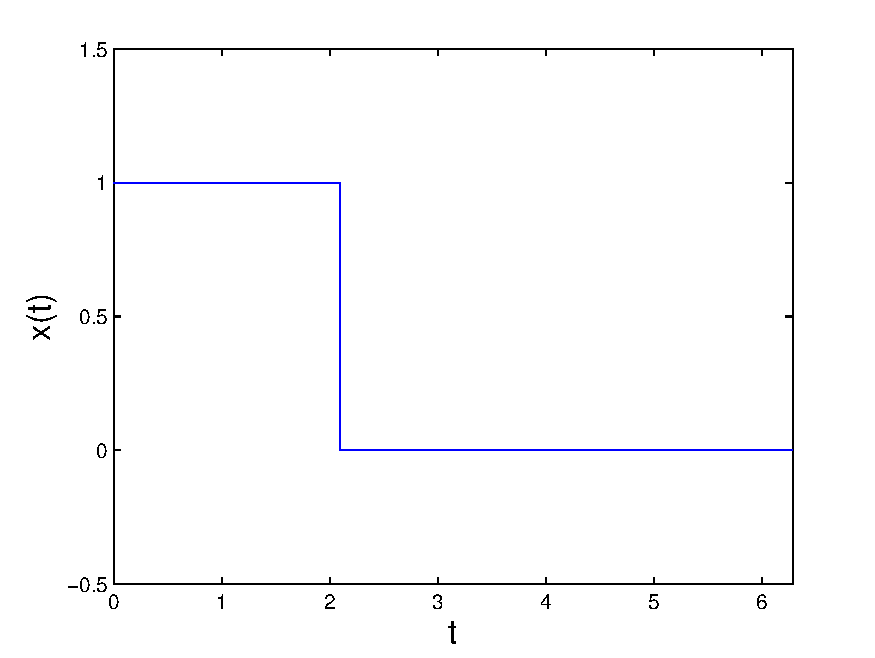
\includegraphics[width=0.45\textwidth]{kugel/Dkonstant/Rechteck2_1.pdf}
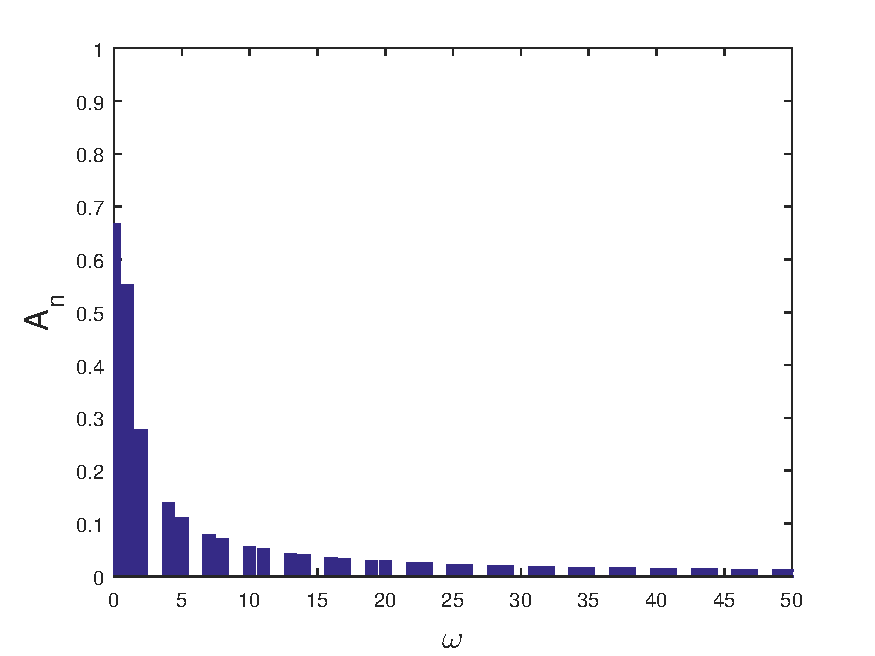
\includegraphics[width=0.45\textwidth]{kugel/Dkonstant/Rechteck2_2.pdf}
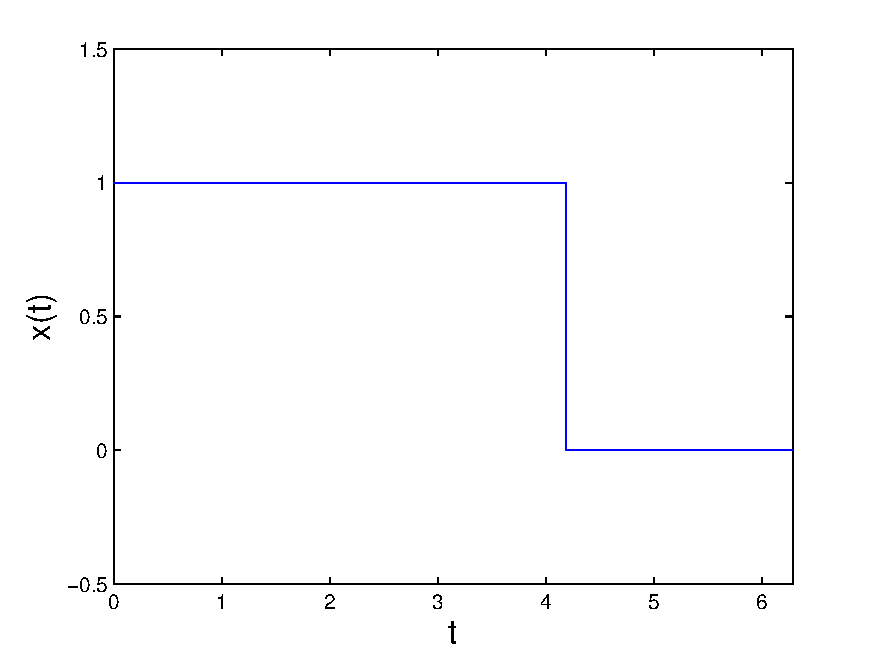
\includegraphics[width=0.45\textwidth]{kugel/Dkonstant/Rechteck3_1.pdf}
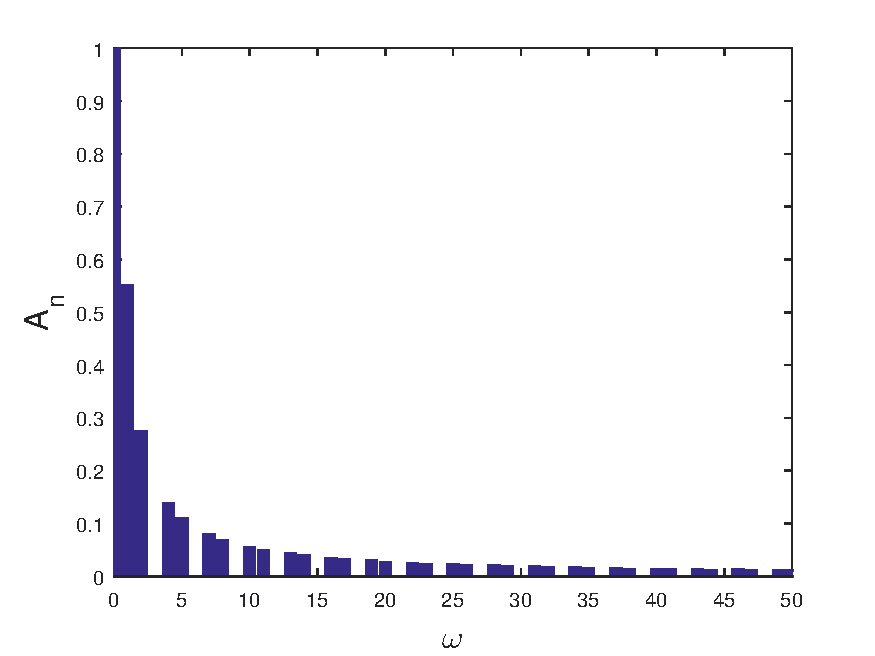
\includegraphics[width=0.45\textwidth]{kugel/Dkonstant/Rechteck3_2.pdf}
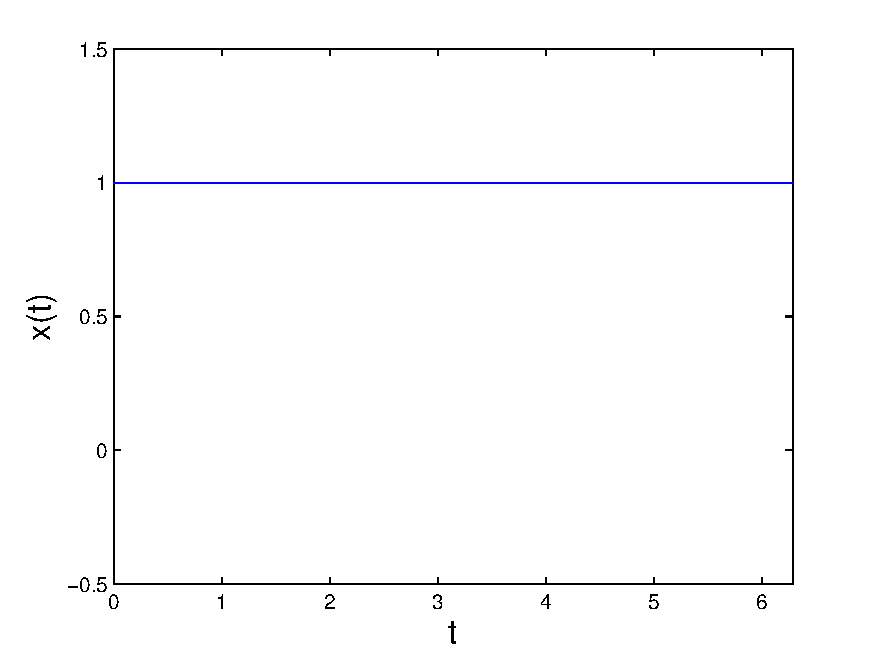
\includegraphics[width=0.45\textwidth]{kugel/Dkonstant/Rechteck4_1.pdf}
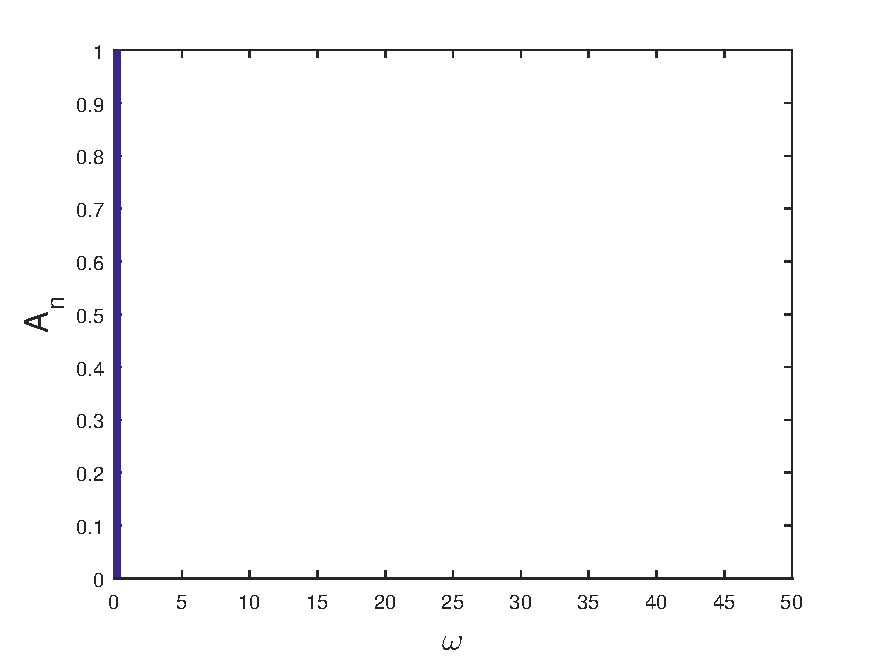
\includegraphics[width=0.45\textwidth]{kugel/Dkonstant/Rechteck4_2.pdf}
\caption{Breiter werdende Rechteckfunktion
\label{skript:Dirac1}}
\end{figure}

\begin{figure}
\centering
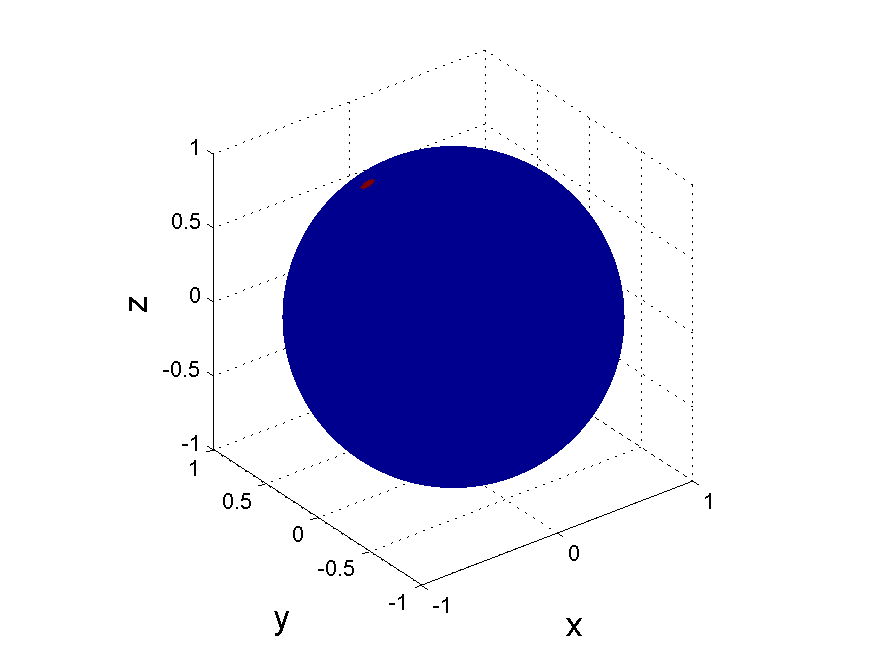
\includegraphics[width=0.45\textwidth]{kugel/Dkonstant/Kugel1_1.pdf}
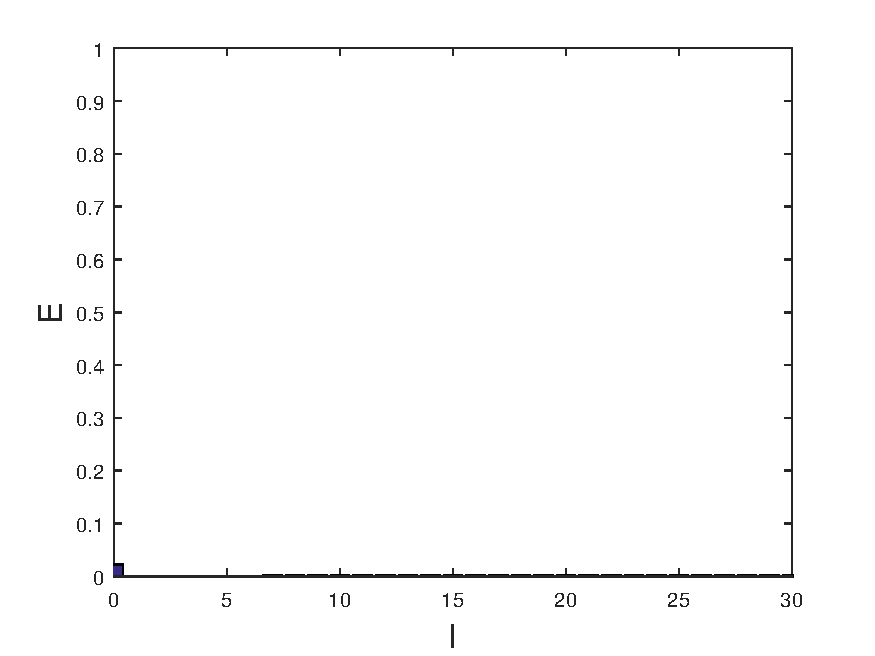
\includegraphics[width=0.45\textwidth]{kugel/Dkonstant/Kugel1_2.pdf}
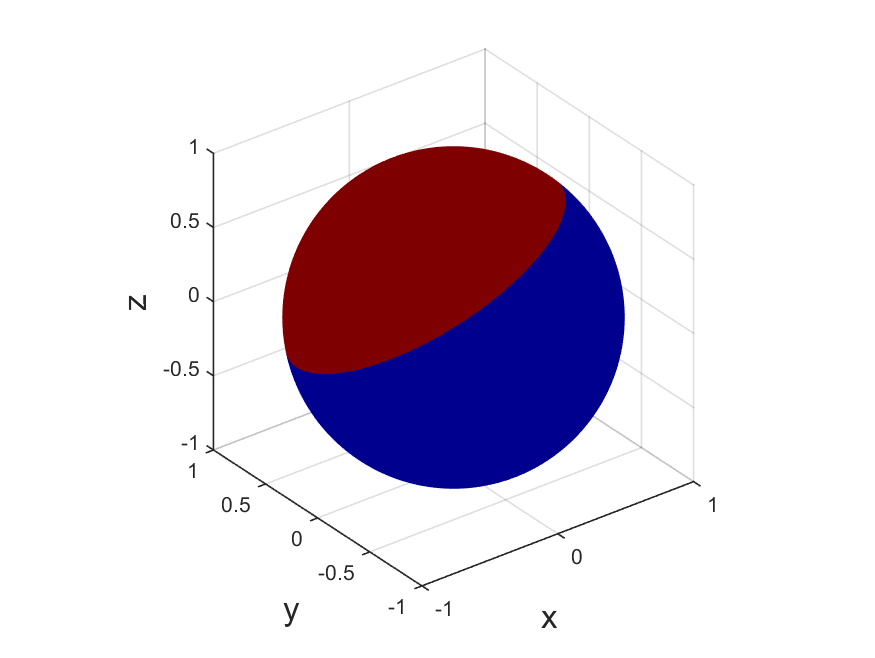
\includegraphics[width=0.45\textwidth]{kugel/Dkonstant/Kugel2_1.pdf}
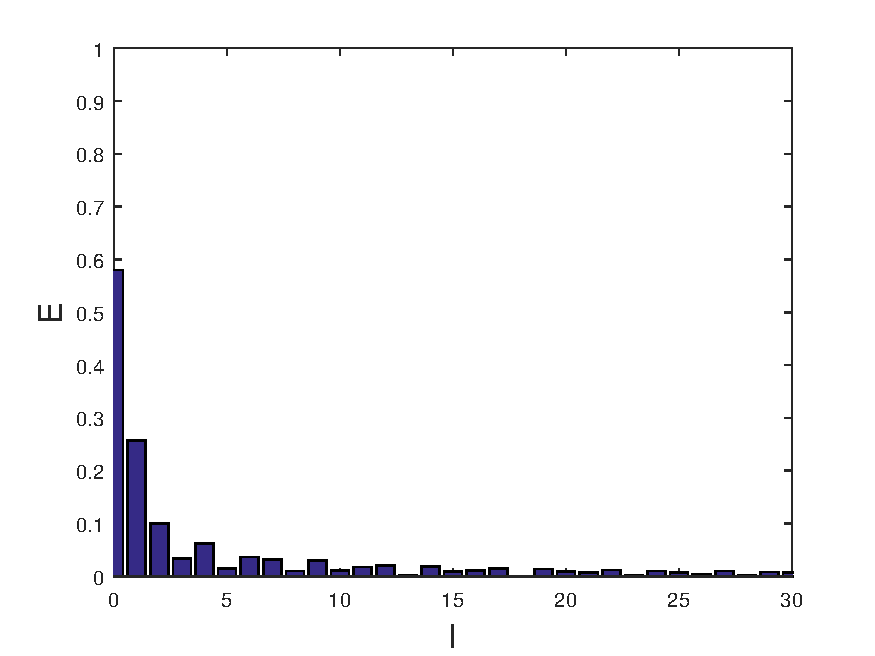
\includegraphics[width=0.45\textwidth]{kugel/Dkonstant/Kugel2_2.pdf}
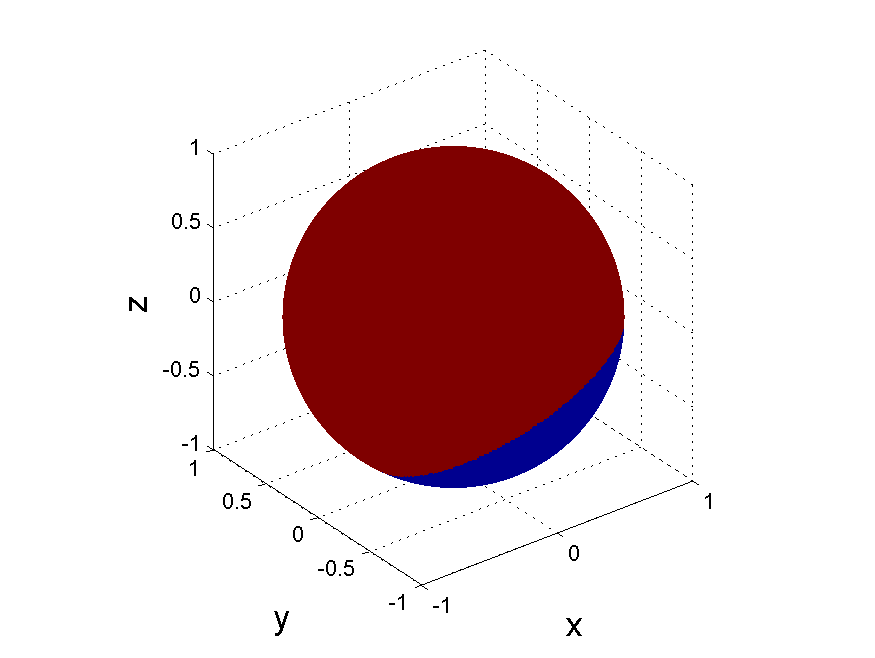
\includegraphics[width=0.45\textwidth]{kugel/Dkonstant/Kugel3_1.pdf}
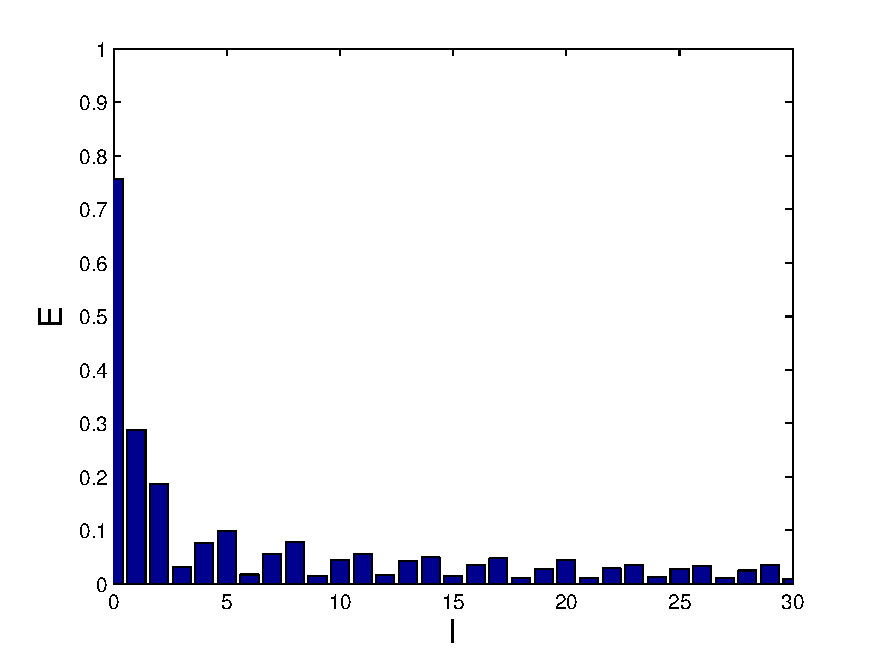
\includegraphics[width=0.45\textwidth]{kugel/Dkonstant/Kugel3_2.pdf}
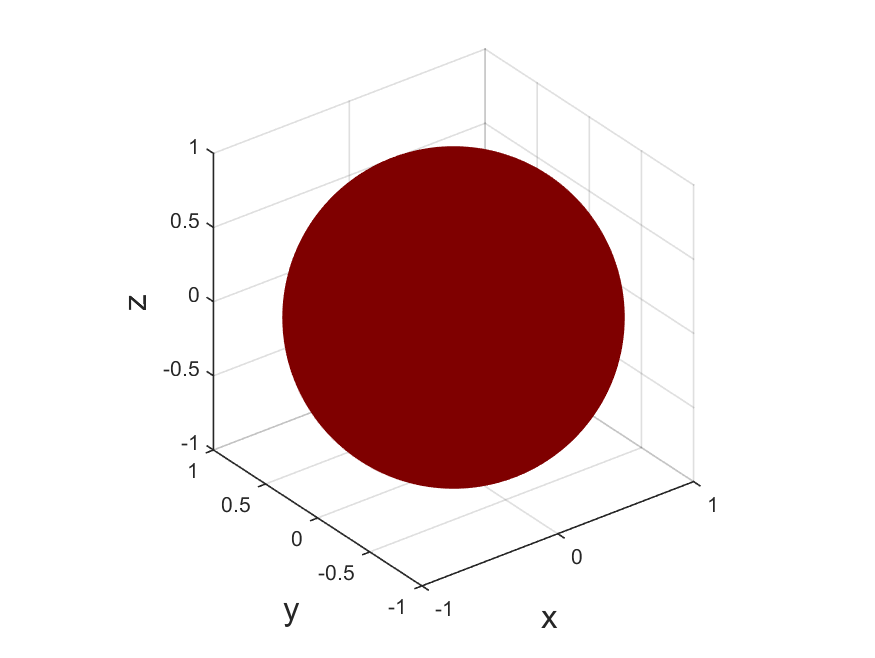
\includegraphics[width=0.45\textwidth]{kugel/Dkonstant/Kugel4_1.pdf}
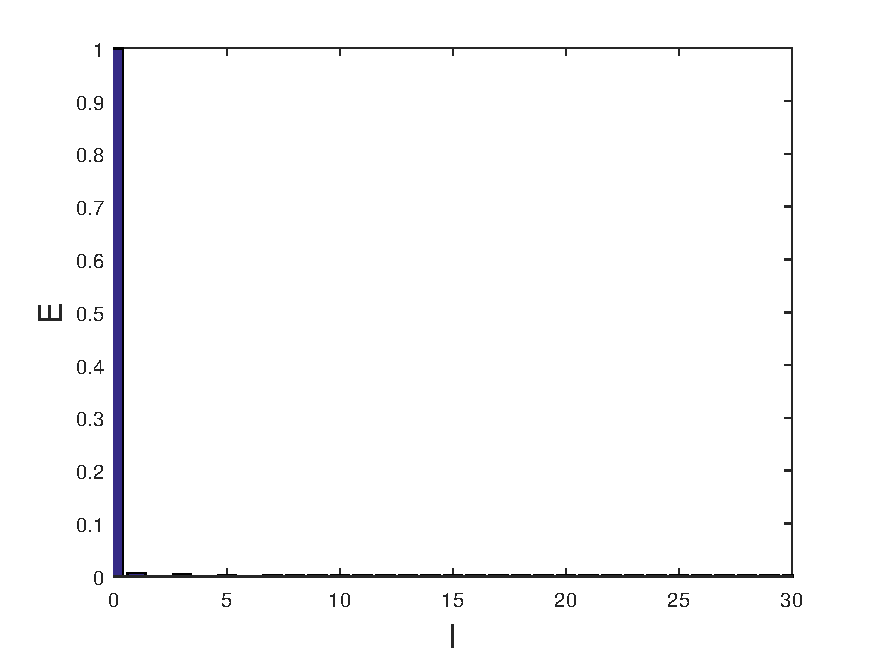
\includegraphics[width=0.45\textwidth]{kugel/Dkonstant/Kugel4_2.pdf}
\caption{Wachsender Kreisabschnitt auf der Kugeloberfl"ache
\label{skript:Dirac2}}
\end{figure}

\section{Gibbs-Ph"anomen}
\rhead{Gibbs-Ph"anomen}
Das Gibbs-Ph"anomen beschreibt, dass man bei der Rekonstruktion einer
Funktion mit Sprungstellen, vor und nach den ursprünglichen Sprungstellen, 
"Uberschwinger von ca. 9\% der Sprunghöhe feststellen kann wenn die 
Bandbreite begrenzt wird. 
Bandbreitenbegrenzung bedeutet, dass nur eine endliche Anzahl 
Fourier-Koeffizienten zur Rekonstruktion einer Funktion verwendet werden. 
Dieses Ph"anomen möchten wir in diesem Abschnitt für periodische 
Funktionen und Funktionen auf der Kugeloberfl"ache beschreiben und 
illustrieren.

\subsection{Gibbs-Ph"anomen bei einer periodischen Funktion}
In Abbildung \ref{skript:Gibborg} ist die Original-Rechteckfunktion 
dargestellt, von welcher wir die Fourier-Koeffizienten berechneten. 
In Abbildung \ref{skript:Gibbsre} ist die, mit den ersten 100 
Fourier-Koeffizienten rekonstruierte Rechteckfunktion zu sehen. 
Es ist deutlich zu erkennen, dass an der Stelle, bei welcher die 
Original-Rechteckfunktion Sprungstellen aufweist, keine Sprungstellen 
mehr vorhanden sind, stattdessen weist die Übergangszone von 0 auf 1 
nur noch eine hohe Flankensteilheit auf und "uberschwingt kurz vor und 
nach den urspr"unglichen Sprungstellen.

\subsection{Gibbs-Ph"anomen bei einer Funktion auf der Kugeloberl"ache}
Dasselbe Ph"anomen ist auch bei Funktionen auf der Kugeloberfl"ache 
zu beobachten. 
In den Abbildungen \ref{skript:Gibbs1} und \ref{skript:Gibbs2} sieht 
man die Originalfunktion auf der Kugeloberfl"ache, von welcher wir, 
wie bei Rechteckfunktion, die Fourier-Koeffizienten berechneten. 
In derselben Abbildung sieht man die rekonstruierten Funktionen auf 
der Kugeloberfl"ache. 
Mit dem Parameter n wird jeweils angegeben wie viele Fourier-
Koeffizienten f"ur die Rekonstruktion der Funktionen verwendet wurden. 
Hier ist gut zu erkennen, dass die "Ubergangszone zwischen 0 und 1 
immer schmaler wird, je mehr Fourier-Koeffizienten für die 
Rekonstruktion verwendet wurden. 
Auch sind die "Uberschwinger vor und nach der urspr"unglichen 
Sprungstelle gut zu erkennen.

\begin{figure}
\begin{minipage}[hbt]{0.5\textwidth}
\centering
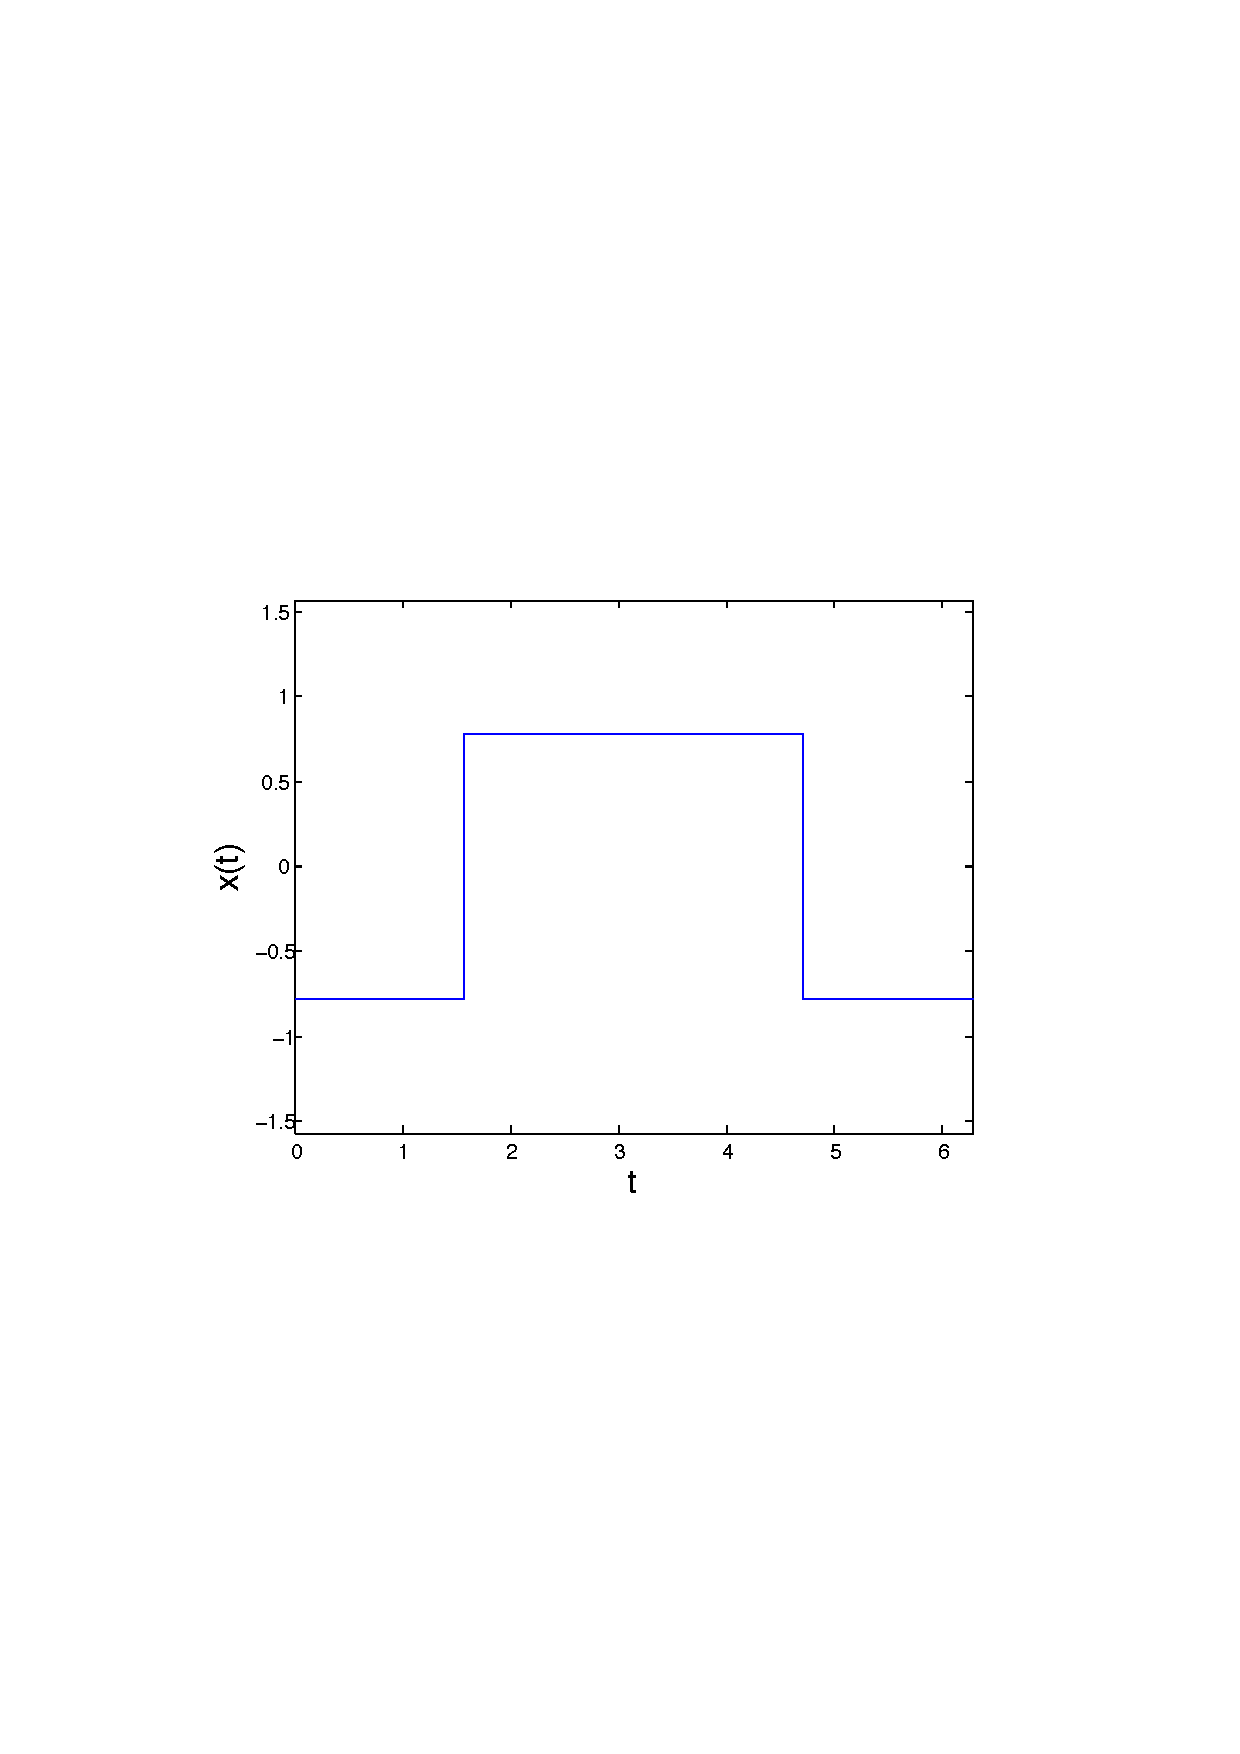
\includegraphics[width=1\textwidth]{kugel/Gibbs/Funktion.pdf}
\caption{Original-Rechteckfunktion}
\label{skript:Gibborg}
\end{minipage}
\hfill
\begin{minipage}[hbt]{0.5\textwidth}
\centering
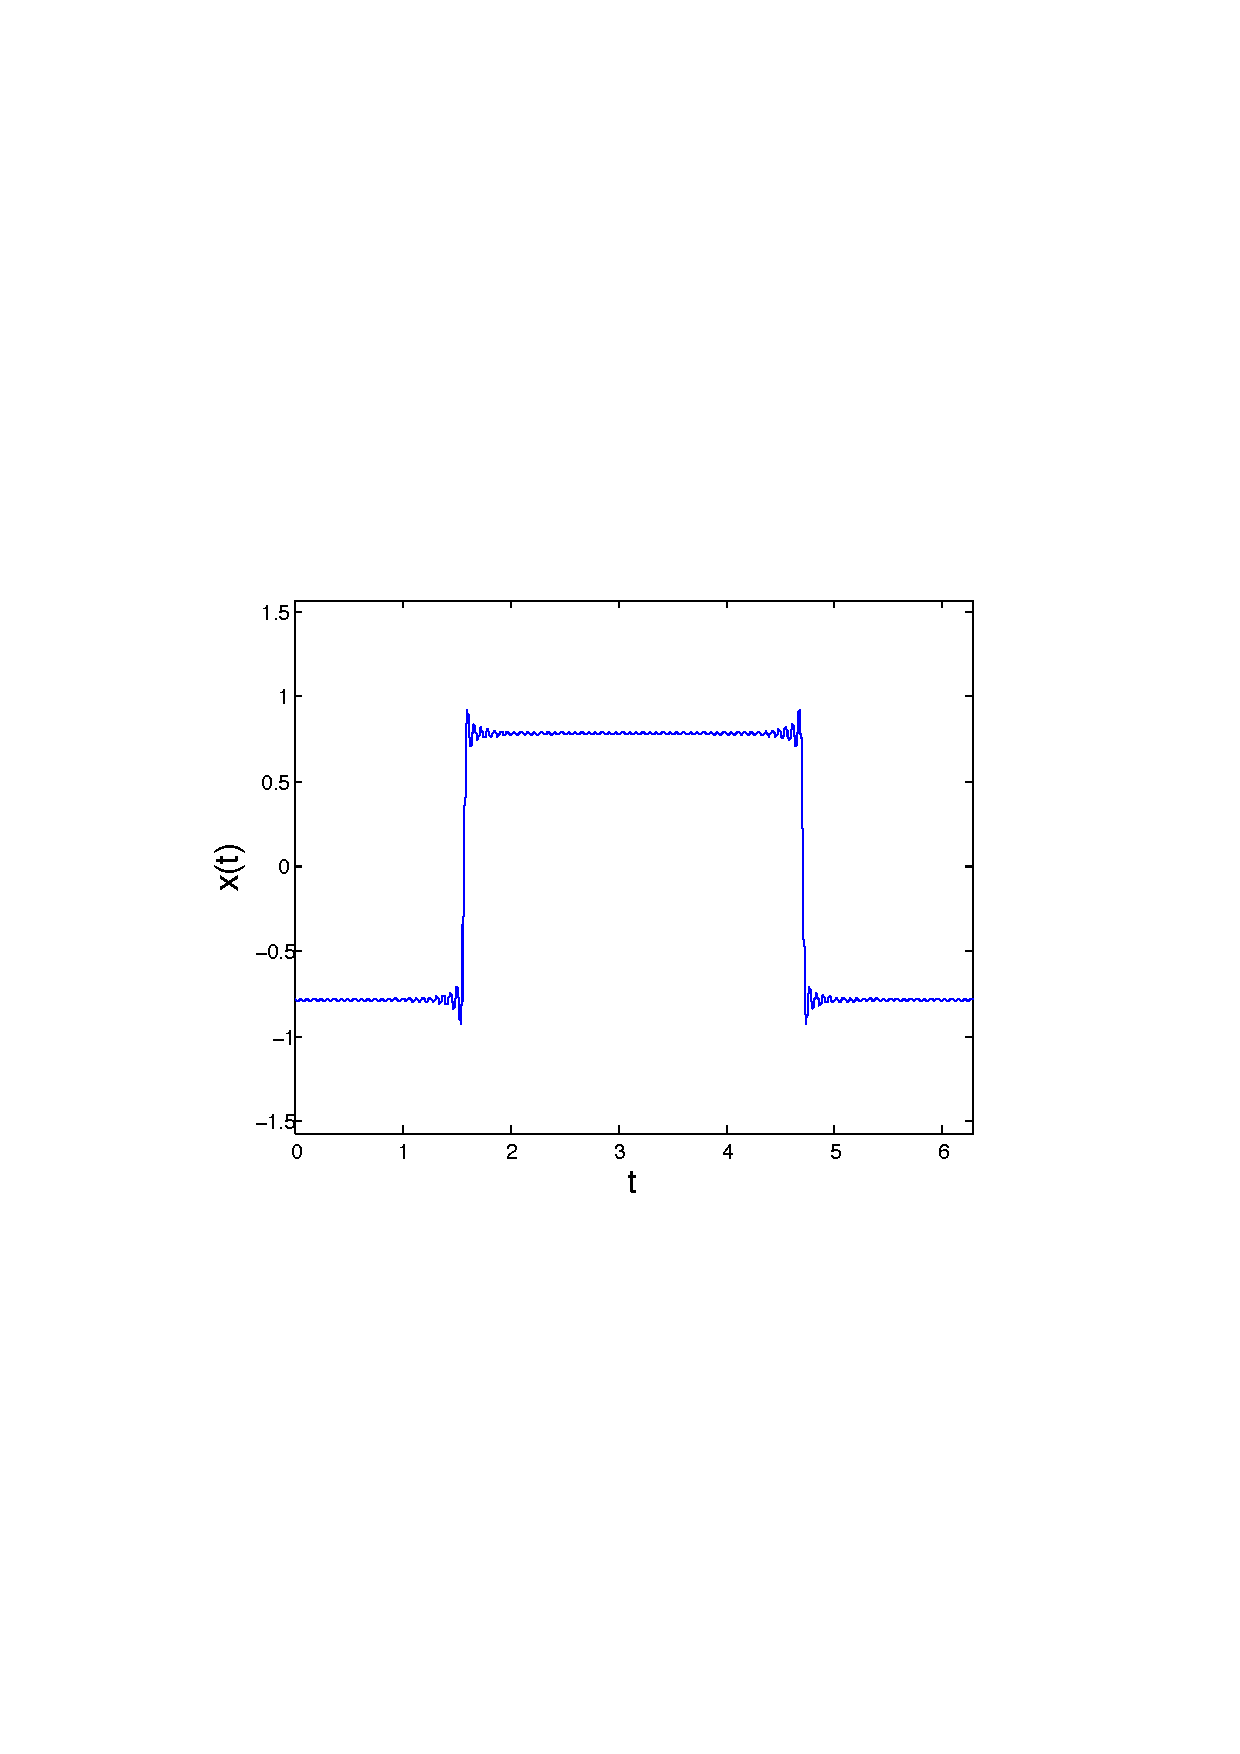
\includegraphics[width=1\textwidth]{kugel/Gibbs/Gibbs.pdf}
\caption{Rekonstruiertes Rechtecksignal}
\label{skript:Gibbsre}
\end{minipage}
\end{figure}

\begin{figure}% Gibbsscher-Effekt
\centering
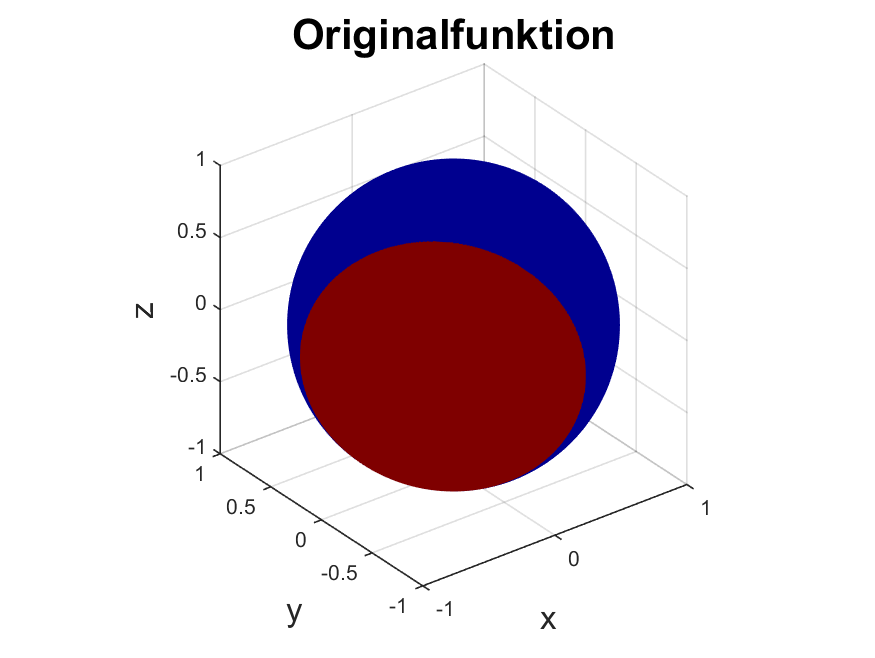
\includegraphics[width=0.4\textwidth]{kugel/Gibbs/GibbsOriginalFunktion.pdf}
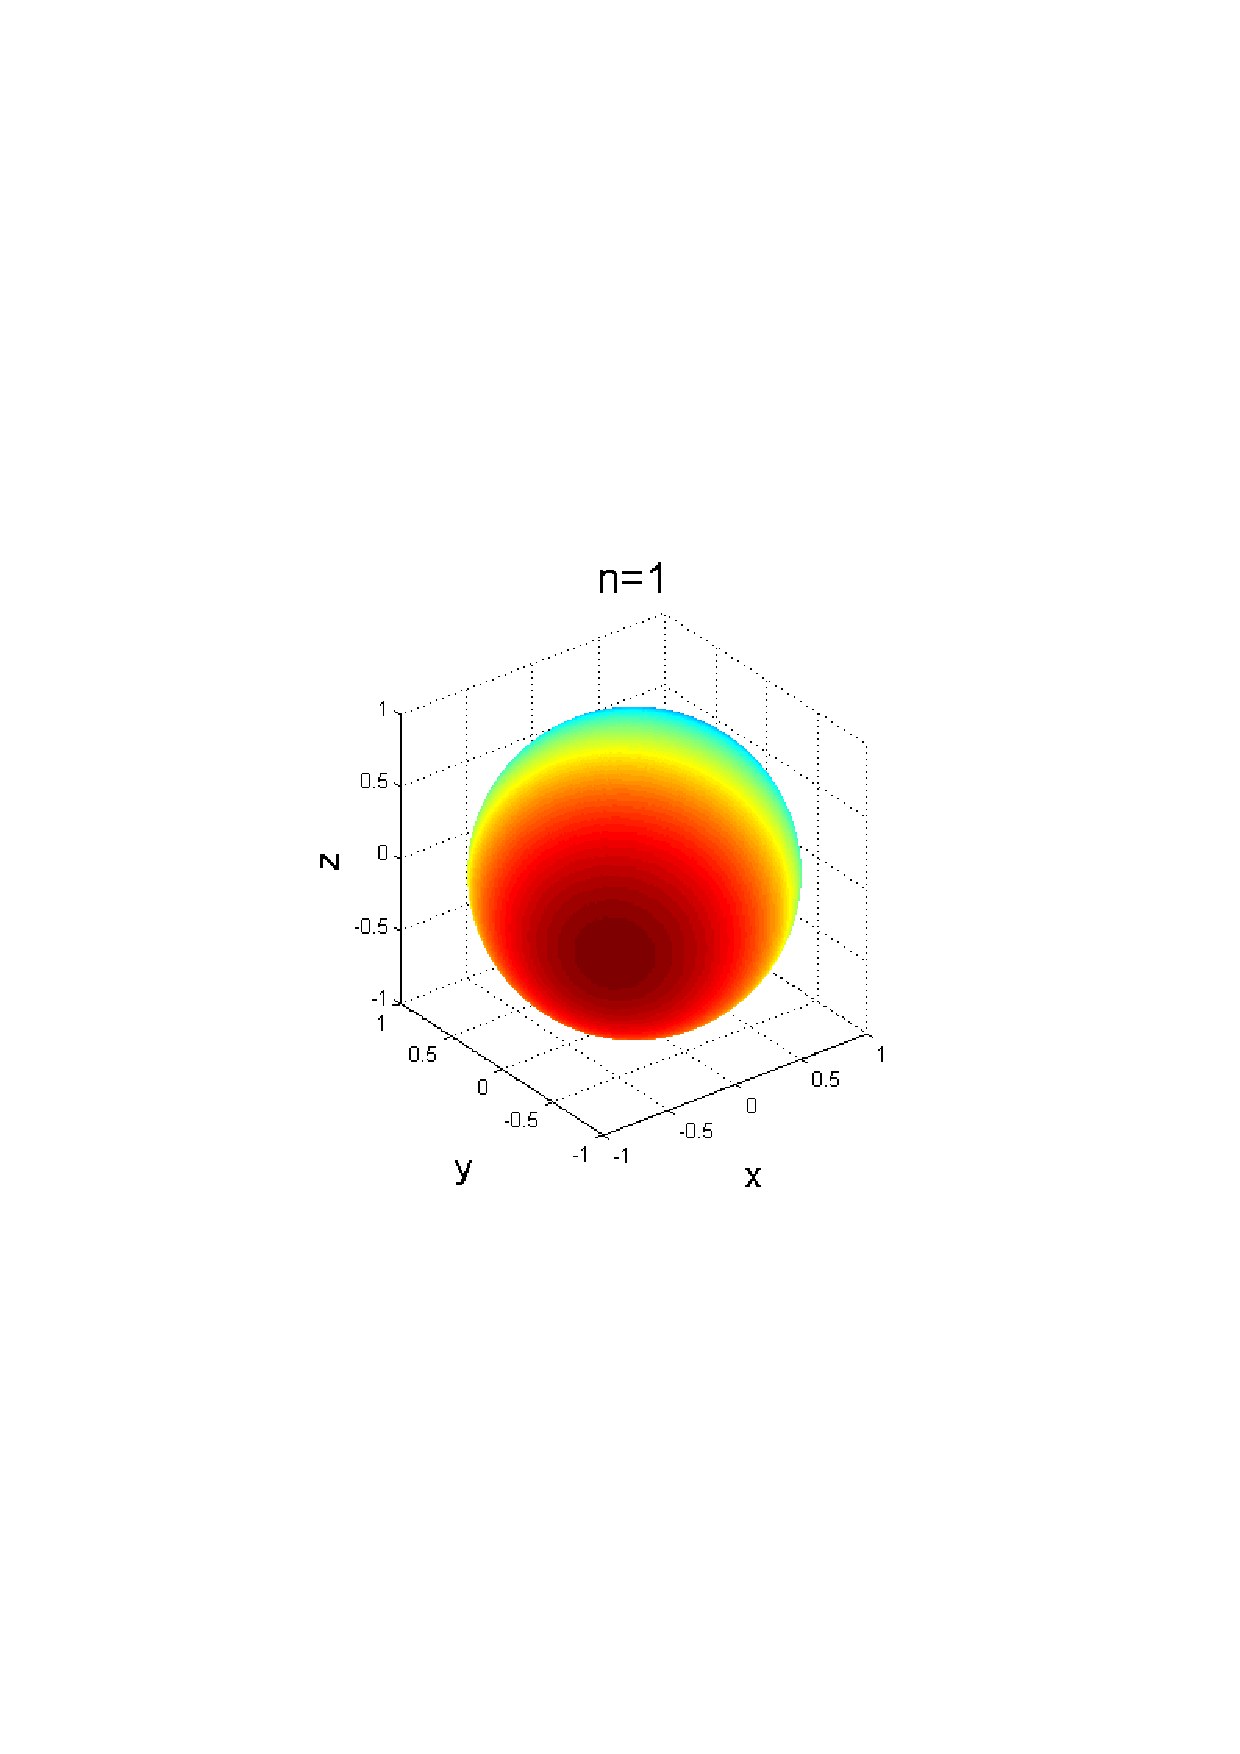
\includegraphics[width=0.4\textwidth]{kugel/Gibbs/GibbsN_1.pdf}
\includegraphics[width=0.4\textwidth]{kugel/Gibbs/GibbsN_2.pdf}
\includegraphics[width=0.4\textwidth]{kugel/Gibbs/GibbsN_3.pdf}
\includegraphics[width=0.4\textwidth]{kugel/Gibbs/GibbsN_4.pdf}
\includegraphics[width=0.4\textwidth]{kugel/Gibbs/GibbsN_5.pdf}
\caption{Gibbs-Ph"anomen mit $n=1$ bis $n=5$
\label{skript:Gibbs1}}
\end{figure}

\begin{figure}% Gibbsscher-Effekt
\centering22
\includegraphics[width=0.4\textwidth]{kugel/Gibbs/GibbsOriginalFunktion.pdf}
\includegraphics[width=0.4\textwidth]{kugel/Gibbs/GibbsN_10.pdf}
\includegraphics[width=0.4\textwidth]{kugel/Gibbs/GibbsN_15.pdf}
\includegraphics[width=0.4\textwidth]{kugel/Gibbs/GibbsN_20.pdf}
\includegraphics[width=0.4\textwidth]{kugel/Gibbs/GibbsN_25.pdf}
\includegraphics[width=0.4\textwidth]{kugel/Gibbs/GibbsN_30.pdf}
\caption{Gibbs-Ph"anomen mit $n=10$ bis $n=30$
\label{skript:Gibbs2}}
\end{figure}

\printbibliography[heading=subbibliography]
\end{refsection}
